%%%%%%%%%%%%%%%%%%%%%%%%%%%%%%%%%%%%%%%%%%%%%%%%%%%%%%%%%%%%%%%%%%%%%%%%%%%%%
% parámetros para configurar el formato del código en los entornos lstlisting
%%%%%%%%%%%%%%%%%%%%%%%%%%%%%%%%%%%%%%%%%%%%%%%%%%%%%%%%%%%%%%%%%%%%%%%%%%%%%
\lstset{ %
    backgroundcolor=\color{white},   % choose the background color; you must add \usepackage{color} or \usepackage{xcolor}
    basicstyle=\footnotesize,        % the size of the fonts that are used for the code
    breakatwhitespace=false,         % sets if automatic breaks should only happen at whitespace
    breaklines=true,                 % sets automatic line breaking
    captionpos=b,                    % sets the caption-position to bottom
    commentstyle=\color{mygreen},    % comment style
    deletekeywords={...},            % if you want to delete keywords from the given language
    %escapeinside={\%*}{*)},          % if you want to add LaTeX within your code
    %extendedchars=true,              % lets you use non-ASCII characters; for 8-bits encodings only, does not work with UTF-8
    %frame=single,	                % adds a frame around the code
    keepspaces=true, keywordstyle=\color{blue}, language=[ANSI]C, % keeps spaces in text, useful for keeping indentation of code (possibly needs columns=flexible)% keyword style% the language of the code
    %otherkeywords={*,...},           % if you want to add more keywords to the set
    numbers=left, numbersep=5pt, numberstyle=\tiny\color{mygray},
    rulecolor=\color{black}, showspaces=false, showstringspaces=false,
    showtabs=false, stepnumber=1, stringstyle=\color{mymauve}, tabsize=2,
    title=\lstname, morecomment=[s]{/*}{*/} }% where to put the line-numbers; possible values are (none, left, right)% how far the line-numbers are from the code% the style that is used for the line-numbers% if not set, the frame-color may be changed on line-breaks within not-black text (e.g. comments (green here))% show spaces everywhere adding particular underscores; it overrides 'showstringspaces'% underline spaces within strings only% show tabs within strings adding particular underscores% the step between two line-numbers. If it's 1, each line will be numbered% string literal style% sets default tabsize to 2 spaces% show the filename of files included with \lstinputlisting; also try caption instead of title

\lstdefinelanguage{PythonUTF8}[]{Python}{
literate={á}{{\'a}}1 {é}{{\'e}}1 {í}{{\'i}}1 {ó}{{\'o}}1 {ú}{{\'u}}1
{Á}{{\'A}}1 {É}{{\'E}}1 {Í}{{\'I}}1 {Ó}{{\'O}}1 {Ú}{{\'U}}1
{ñ}{{\~n}}1 {Ñ}{{\~N}}1
}

\definecolor{mygreen}{rgb}{0,0.6,0}
\definecolor{mygray}{rgb}{0.5,0.5,0.5}
\definecolor{mymauve}{rgb}{0.58,0,0.82}

\chapter{Diseño e implementación} % Main chapter title

\label{Chapter3} % Change X to a consecutive number; for referencing this chapter elsewhere, use \ref{ChapterX}

Este capítulo describe el diseño y la implementación del sistema de monitoreo y
control de invernaderos. Se detallan los componentes principales del sistema,
las decisiones de diseño tomadas y los pasos seguidos para su implementación.

%----------------------------------------------------------------------------------------
%	SECTION 1
%----------------------------------------------------------------------------------------
\section{Arquitectura del sistema}

La figura \ref{fig:arquitectura} ilustra la arquitectura general del sistema y
la interacción entre los diferentes componentes.

\begin{figure}[H]
    \centering
    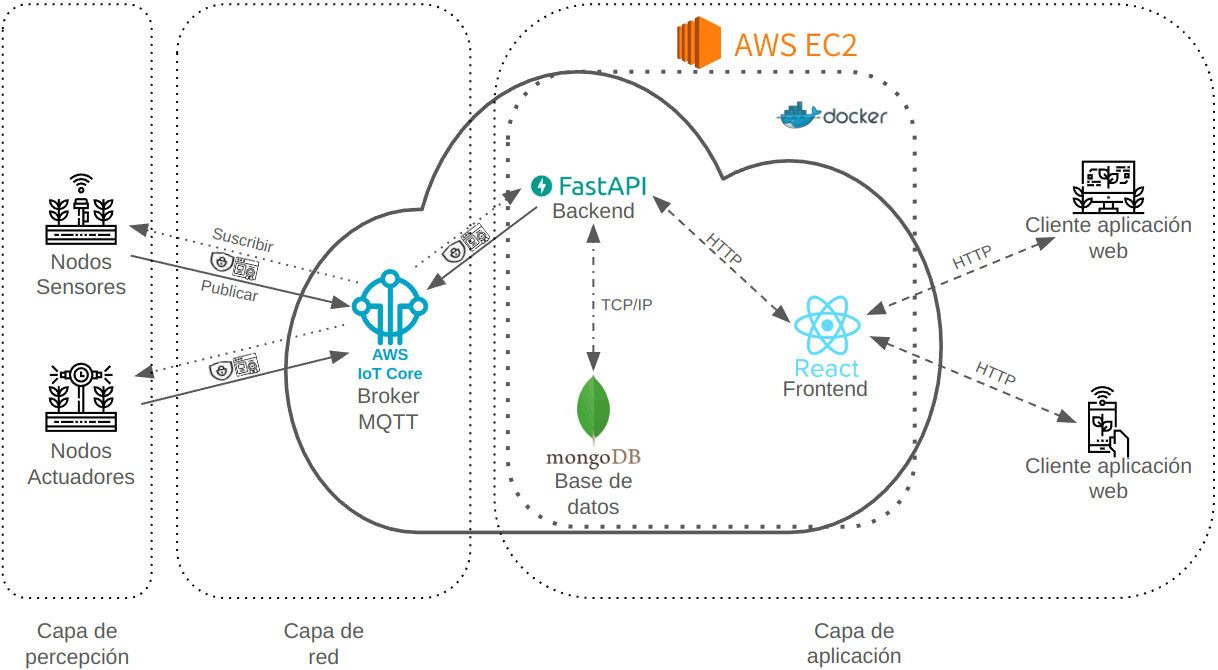
\includegraphics[width=.99\textwidth]{./Images/14.png}
    \caption{Arquitectura de la solución propuesta.}
    \label{fig:arquitectura}
\end{figure}

La arquitectura planteada para el desarrollo del trabajo sigue el modelo de
tres capas típico de un sistema IoT: percepción, red y aplicación.

\subsection{Capa de percepción}

La capa de percepción está constituida por los nodos sensores y actuadores, que
se encargan de recopilar datos del entorno y ejecutar acciones específicas en
función de los parámetros configurados.

Cada nodo sensor incluye un microcontrolador ESP-WROOM-32, este se conecta a
diversos sensores que miden parámetros como temperatura ambiente, humedad
relativa, presión atmosférica, nivel de iluminación, concentración de $CO_2$,
pH, CE, temperatura de la solución nutritiva, nivel de líquidos, consumo
eléctrico, entre otros. Los nodos actuadores, por su parte, cuentan con relés
para controlar dispositivos como ventiladores, iluminación y sistemas de
recirculación de nutrientes.

Los nodos fueron conectados a una red Wi-Fi local, lo que les permitió
establecer comunicación con la red y transmitir los datos hacia el servidor IoT
mediante el protocolo MQTT.

\subsection{Capa de red}

La capa de red está conformada por la infraestructura que gestiona la
comunicación entre los nodos del sistema (sensores y actuadores) y la
plataforma en la nube. Una vez integrados a la red local, los nodos emplearon
el protocolo MQTT para publicar y recibir datos de manera eficiente.

El broker MQTT utilizado en este trabajo es AWS IoT Core, un servicio
completamente gestionado que permite establecer una conexión segura y escalable
entre los dispositivos IoT y la nube. Este broker actúa como intermediario para
la transmisión de datos entre los nodos y la capa de aplicación.

La comunicación entre los nodos y el broker MQTT se aseguró mediante el uso de
certificados generados en el propio broker, los cuales garantizaron la
autenticación de los dispositivos y el cifrado de los datos.

\subsection{Capa de aplicación}

La capa de aplicación es responsable del procesamiento, almacenamiento y
visualización de los datos recopilados por los nodos. Para esta capa, se
implementó el servidor IoT en la nube a través del servicio AWS EC2, que
permite ejecutar aplicaciones y servicios en instancias virtuales.

El procesamiento de los datos se llevó a cabo mediante un backend desarrollado
con FastAPI, encargado de gestionar las solicitudes e interactuar con la base
de datos MongoDB, utilizada para el almacenamiento de la información.

Además, se desarrolló una interfaz de usuario en React que permite la
visualización y gestión de los datos de manera intuitiva y accesible desde
cualquier dispositivo con conexión a internet.

Todos los servicios fueron desplegados en contenedores Docker y orquestados
mediante Docker Compose \cite{DockerCompose}, lo que permitió una gestión
eficiente, modular y escalable de los distintos componentes del sistema.

%----------------------------------------------------------------------------------------
%	SECTION 2
%----------------------------------------------------------------------------------------
\section{Modelo de datos}

En esta sección se presenta el modelo de datos implementado en el sistema.

La figura \ref{fig:modelo de datos} permite visualizar las principales
colecciones y sus relaciones dentro de la base de datos. El diseño del modelo
de datos se desarrolló en base a los tipos de datos proporcionados por los
sensores, así como los requerimientos técnicos establecidos para el sistema.

\begin{figure}[H]
    \centering
    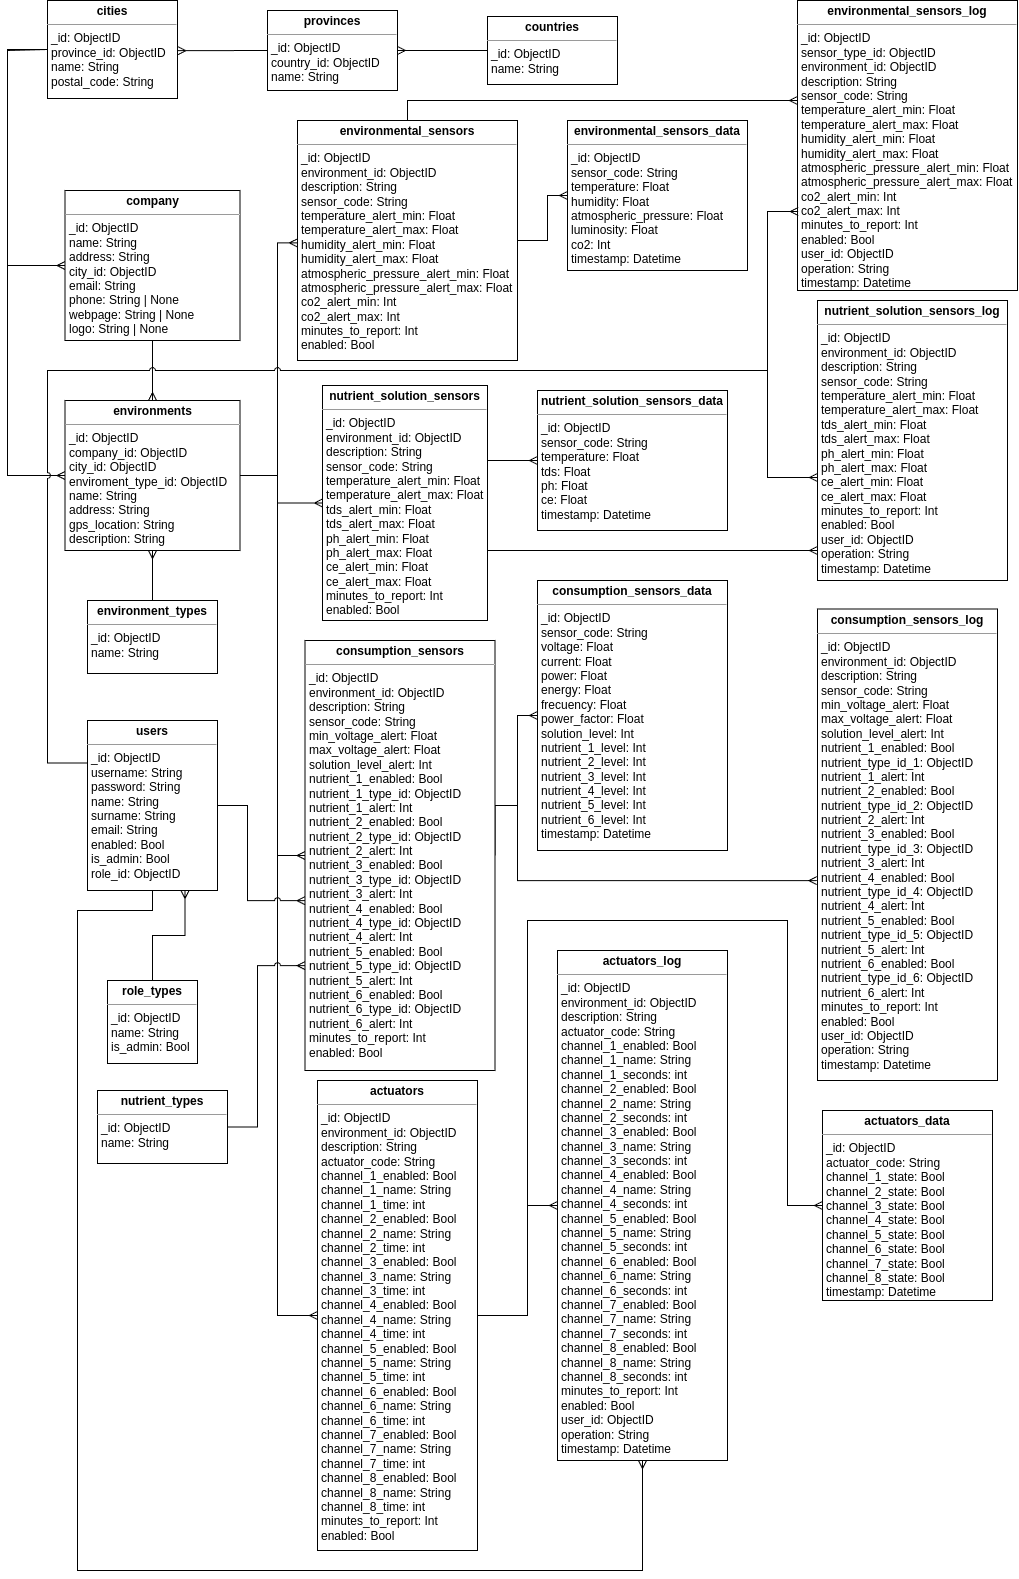
\includegraphics[width=.99\textwidth]{./Images/15.png}
    \caption{Modelo de datos implementado.}
    \label{fig:modelo de datos}
\end{figure}

El modelo de datos se estructuró en colecciones dentro de MongoDB, organizadas
en las siguientes categorías principales:

\subsection{Parametrización del sistema}

\begin{itemize}
    \item Colecciones de configuración básica: países, provincias, ciudades, empresa.
    \item Colecciones para gestión de espacios: ambientes y tipos de ambientes.
    \item Colecciones específicas del dominio: tipos de nutrientes.
\end{itemize}

\subsection{Gestión de usuarios y roles}

\begin{itemize}
    \item Colección de usuarios: almacena información de los usuarios y sus credenciales.
    \item Colección de roles: se plantea como futura funcionalidad, para poder
          parametrizar permisos para cada tipo de rol.
\end{itemize}

\subsection{Sensores y actuadores}
\begin{itemize}
    \item Colecciones de sensores y actuadores: almacena la información de cada tipo de
          dispositivo, los parámetros de alerta y la frecuencia de muestreo.
    \item Colecciones de datos históricos: registran las mediciones vinculadas a cada
          dispositivo mediante identificadores únicos.
\end{itemize}

\subsection{Auditoría y seguimiento}
\begin{itemize}
    \item Colecciones de logs: permiten registrar los cambios en las configuraciones de
          sensores y actuadores realizados por los usuarios.
\end{itemize}

El modelo de datos completo del sistema, puede consultarse en el apéndice
\ref{AppendixA}.

%----------------------------------------------------------------------------------------
%	SECTION 3
%----------------------------------------------------------------------------------------
\section{Servidor IoT}

En esta sección se presenta la arquitectura del sistema y del servidor, junto
con las tecnologías utilizadas.

\subsection{Arquitectura del servidor}

\label{sec:arquitecturaServidor}

La arquitectura del servidor está compuesta por tres componentes principales:
backend, almacenamiento y frontend, como se muestra en la figura
\ref{fig:arquitectura servidor}.

\begin{figure}[H]
    \centering
    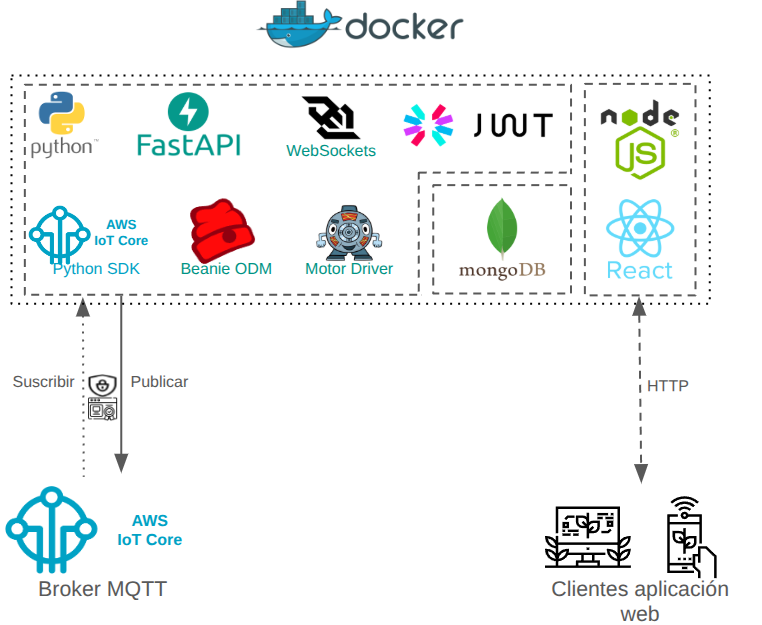
\includegraphics[width=\textwidth]{./Images/16.png}
    \caption{Arquitectura del servidor del sistema IoT.}
    \label{fig:arquitectura servidor}
\end{figure}

A continuación, se describe brevemente cada uno de estos componentes:

\begin{itemize}
    \item Backend: implementado en FastAPI, expone una API REST que permite gestionar
          sensores, actuadores, ambientes y usuarios. Incluye autenticación y
          autorización basada en JWT, integración con MongoDB a través de Beanie
          \cite{BeaniODM} y Motor \cite{MotorMongoDB}, conexión con el broker MQTT
          implementada con el SDK (del inglés, \textit{Software Development Kit}) de AWS
          IoT para Python \cite{AWSIoTSDK} y soporte para comunicaciones en tiempo real
          con clientes mediante WebSocket \cite{FastAPIWebSockets}.

    \item Almacenamiento: utiliza MongoDB como base de datos NoSQL. La información se
          organiza en colecciones para almacenar datos de sensores, actuadores, usuarios,
          ambientes y registros de configuración.

    \item Frontend: desarrollado en React, permite a los usuarios visualizar datos en
          tiempo real, reportes y configurar el sistema. Se conecta con la API REST del
          backend y utiliza WebSocket para actualizaciones en tiempo real.
\end{itemize}

%----------------------------------------------------------------------------------------
%	SECTION 4
%----------------------------------------------------------------------------------------
\section{Desarrollo del backend}

En esta sección se detallan los aspectos clave en el diseño y desarrollo del
servidor backend, así como la lógica de negocio implementada.

\subsection{Diseño de la API}

El diseño se estructuró en base a las necesidades del sistema y los
requerimientos establecidos. Se organizaron los archivos en carpetas de acuerdo
a su funcionalidad.

La tabla \ref{tab:endpoints} presenta un resumen de los principales endpoints
de la API, junto con una breve descripción de la acción y el método HTTP
utilizado.

\begin{table}[H]
    \centering
    \caption[Resumen de los principales endpoints de la API]{Resumen de los principales endpoints de la API.}
    \begin{tabular}{l l l}
        % \begin{tabular}{p{1.3cm}p{5.7cm}p{4.9cm}}
        \toprule
        \textbf{Método} & \textbf{Endpoint}                 & \textbf{Acción}             \\
        \midrule
        GET             & /mqtt/test                        & Test conexión cliente MQTT. \\
        POST            & /mqtt/publish                     & Publicar en tópico MQTT.    \\
        \midrule
        POST            & /login                            & Login de usuarios.          \\
        GET             & /renew-token                      & Renovar token.              \\
        \midrule
        GET             & /users/                           & Obtener usuarios.           \\
        \midrule
        GET             & /environments/                    & Obtener ambientes.          \\
        \midrule
        GET             & /actuators/                       & Obtener actuadores.         \\
        \midrule
        GET             & /sensors/environmental/           & Obtener sensores.           \\
        \midrule
        GET             & /sensors/nutrients/solution/      & Obtener sensores.           \\
        \midrule
        GET             & /sensors/consumption/             & Obtener sensores.           \\
        \midrule
        GET             & /actuators/data/                  & Obtener datos históricos.   \\
        GET             & /sensors/environmental/data/      & Obtener datos históricos.   \\
        GET             & /sensors/consumption/data/        & Obtener datos históricos.   \\
        GET             & /sensors/nutrients/solution/data/ & Obtener datos históricos.   \\
        \bottomrule
        \hline
    \end{tabular}
    \label{tab:endpoints}
\end{table}

El listado completo de endpoints de la API se puede consultar en el apéndice
\ref{AppendixB}.

\subsection{Autenticación y autorización}

Se implementó un sistema de autenticación basado en JWT, que permite a los
usuarios acceder a la API de manera segura. La autenticación se realiza
mediante el envío de las credenciales del usuario en el cuerpo de la solicitud,
y el servidor responde con un token JWT que se utiliza para autenticar las
solicitudes posteriores.

El token contiene la información del usuario y se envía en el encabezado de las
solicitudes a la API. El servidor verifica su validez y, en función de ello,
permite o deniega el acceso a los recursos solicitados.

Dado que el token fue diseñado con un tiempo de expiración, se implementó un
mecanismo de renovación que permite a los usuarios mantener la sesión activa
sin necesidad de volver a autenticarse con sus credenciales.

La figura \ref{fig:esquema autenticacion} muestra el esquema de autenticación,
autorización y renovación de token implementado en el sistema.

\begin{figure}[H]
    \centering
    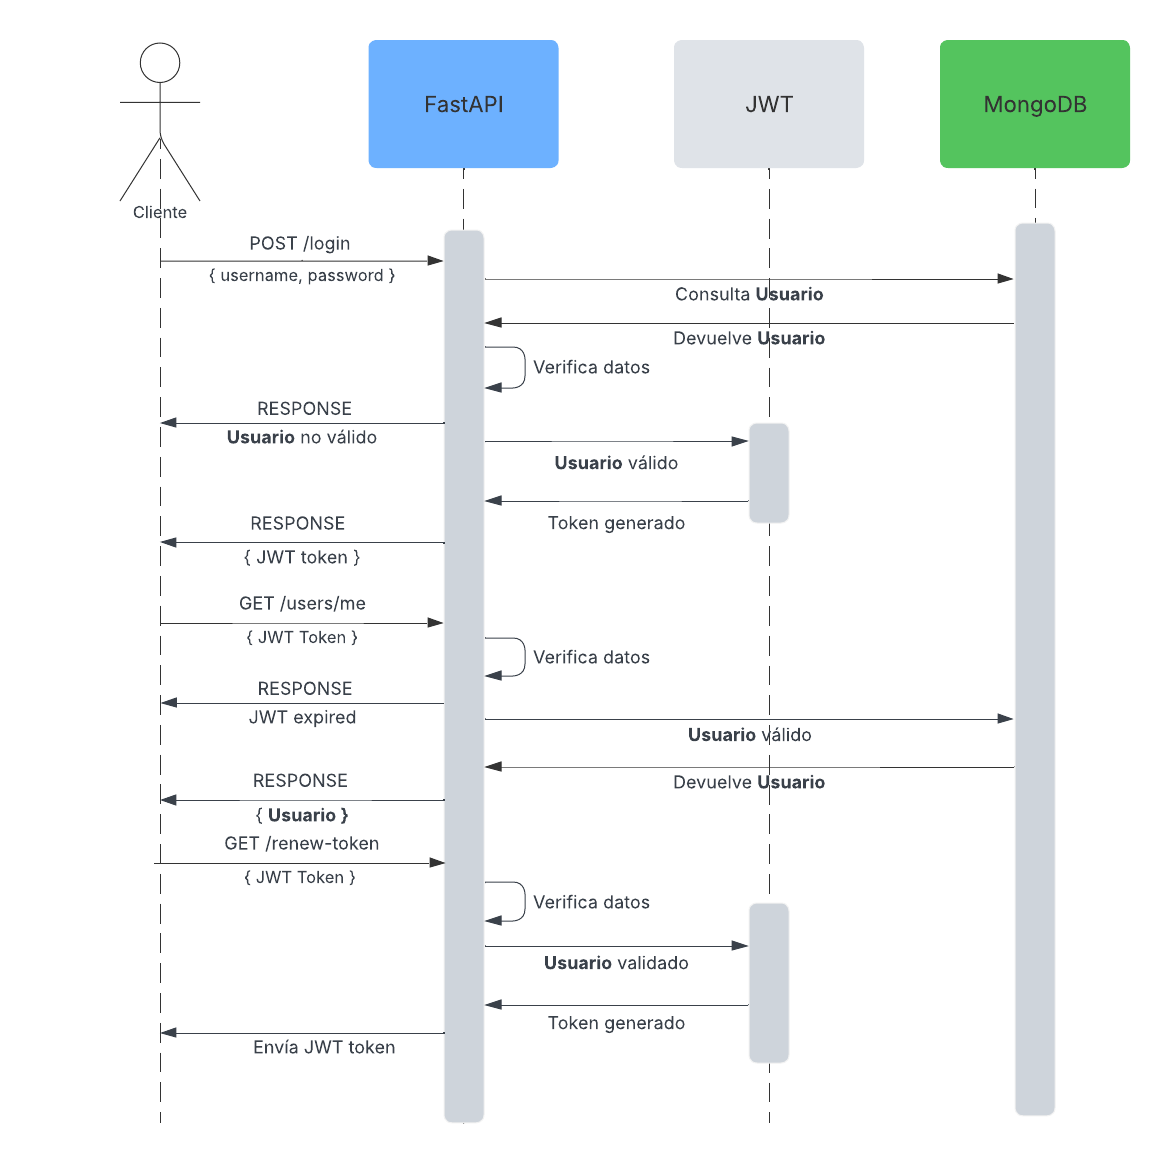
\includegraphics[width=.78\textwidth]{./Images/17.png}
    \caption{Esquema de autenticación y autorización.}
    \label{fig:esquema autenticacion}
\end{figure}

\subsection{Persistencia de datos}

En FastAPI, cada modelo representa una colección en la base de datos e incluye
los campos necesarios para almacenar la información requerida. La comunicación
entre el backend y la base de datos se realizó a través de la biblioteca Motor,
que proporciona una interfaz asíncrona para interactuar con MongoDB. Además se
utilizó el ODM (del inglés, \textit{Object Document Mapper}), a través de la
biblioteca Beanie, que permite definir modelos y realizar consultas y
operaciones sobre la base de datos de manera sencilla.

La figura \ref{fig:diagrama de clases} muestra un ejemplo de la relación entre
los modelos implementados en el sistema y los métodos HTTP de la colección
\texttt{EnvironmentalSensor}.

\begin{figure}[H]
    \centering
    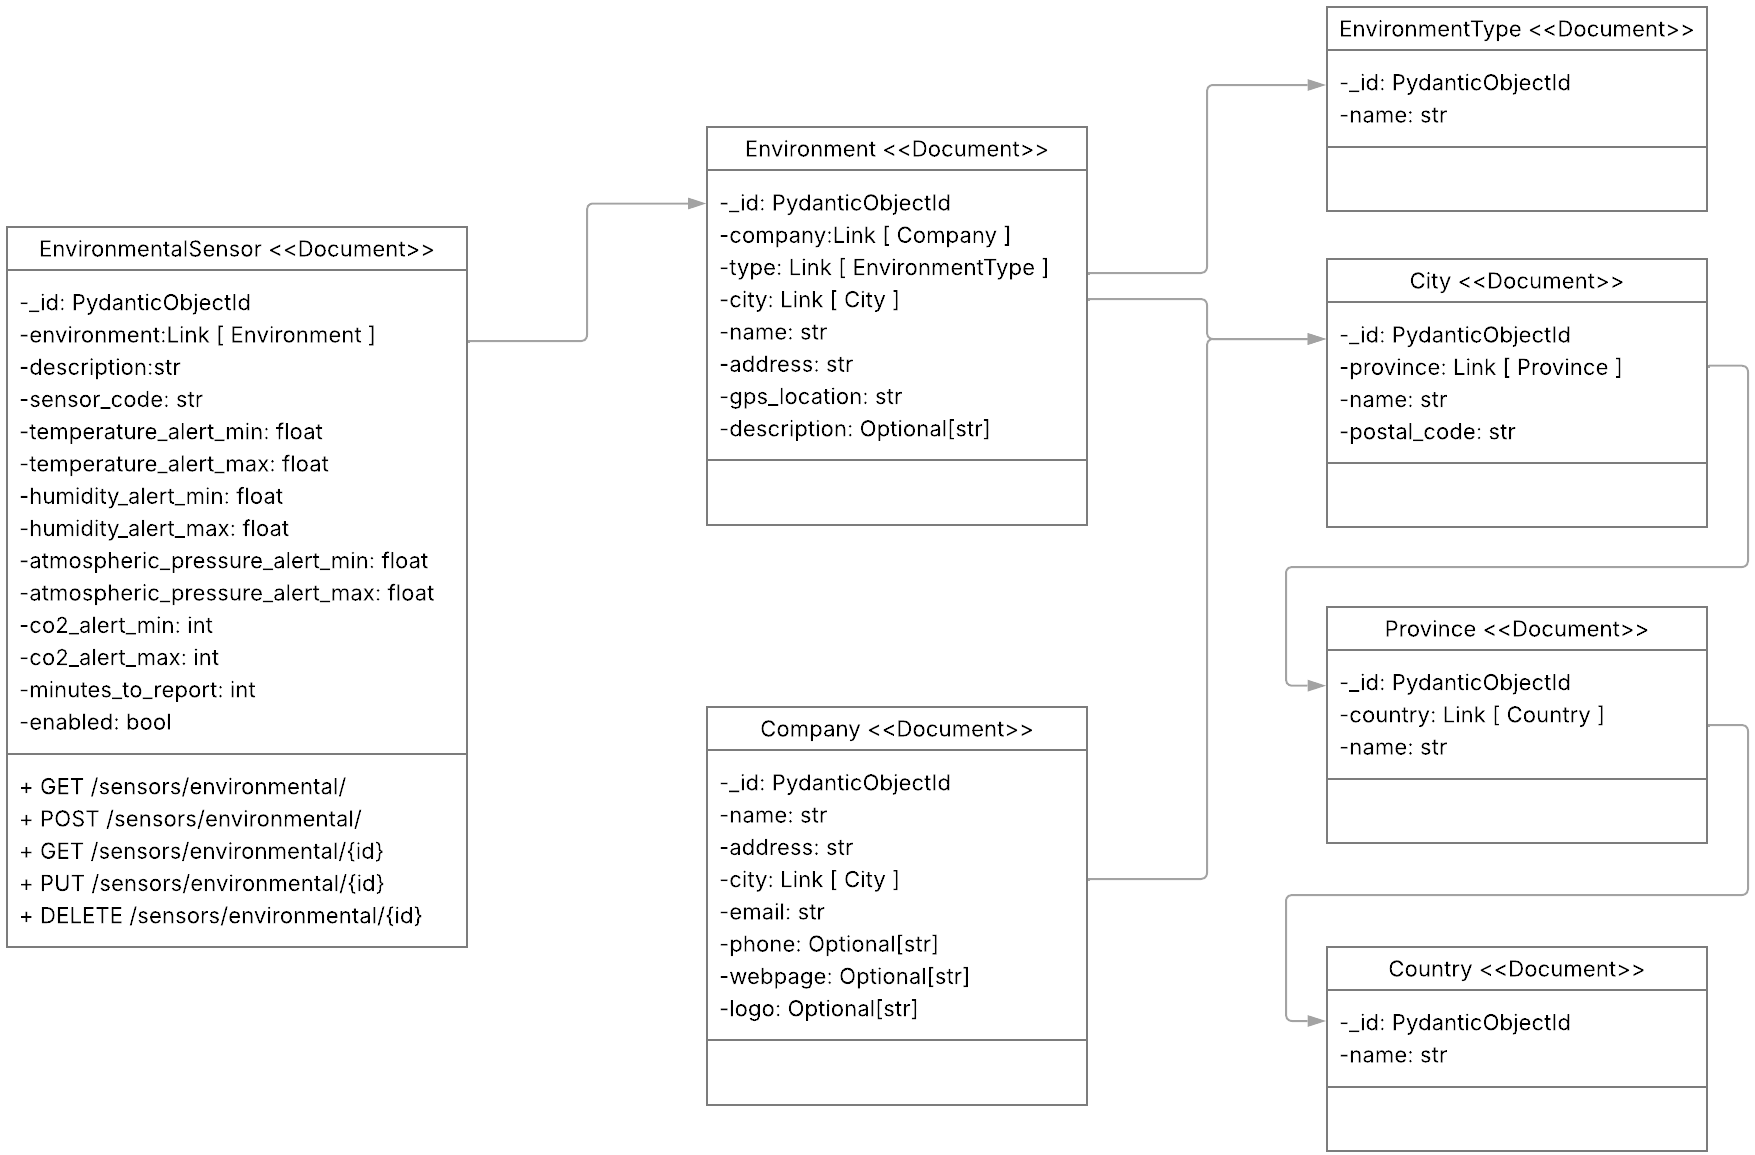
\includegraphics[width=.88\textwidth]{./Images/18.png}
    \caption{Diagrama de clase de la colección \texttt{EnvironmentalSensor}.}
    \label{fig:diagrama de clases}
\end{figure}

Como se mencionó anteriormente, los datos se almacenan en MongoDB. Para
establecer la conexión con la base de datos, se utiliza el cliente asíncrono de
la biblioteca Motor, mientras que la inicialización de los modelos se realiza
mediante la función \texttt{init\_beanie} del ODM Beanie. Esta función
configura los modelos y establece la conexión con la base de datos. En la
cadena de conexión se especifica el nombre de usuario, la contraseña y la
dirección del servidor de MongoDB.

La figura \ref{fig:conexion mongo} ilustra los pasos necesarios para establecer
la conexión entre FastAPI y MongoDB.

\begin{figure}[H]
    \centering
    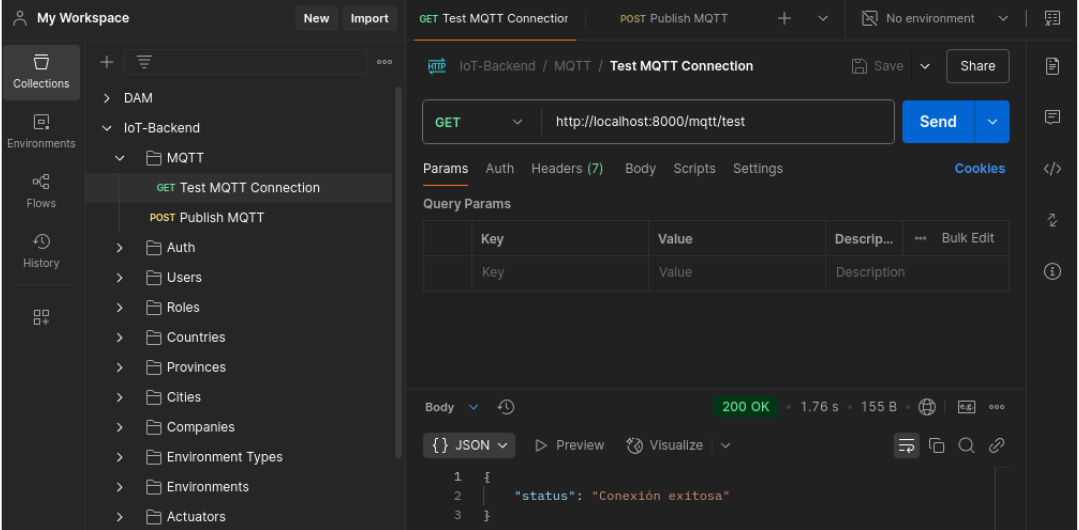
\includegraphics[width=.87\textwidth]{./Images/19.png}
    \caption{Pasos para la conexión de FastAPI y MongoDB.}
    \label{fig:conexion mongo}
\end{figure}

\subsection{Comunicación con el Broker MQTT}

A continuación, se detalla el proceso de implementación de la comunicación con
el broker MQTT en AWS IoT Core.

\subsubsection{Configuración del Thing y Certificados de Seguridad}

Para establecer una conexión segura con el broker MQTT, se realizaron los
siguientes pasos en AWS IoT Core:

\begin{enumerate}
    \item Creación del Thing: se creó un objeto \textit{Thing} en AWS IoT Core, que
          representa un dispositivo IoT. Este objeto se utiliza para gestionar la
          conexión y la comunicación con el broker.

    \item Generación de certificados:
          \begin{itemize}
              \item Se emitieron certificados de seguridad y claves privadas específicas para el
                    \textit{Thing}.
              \item Se descargó el certificado raíz de Amazon CA(del inglés, \textit{Certificate
                        Authority}) para validar la autenticidad del broker.
          \end{itemize}
          Estos elementos permiten:
          \begin{itemize}
              \item Autenticación mutua entre dispositivo y broker.
              \item Cifrado de extremo a extremo de la comunicación.
          \end{itemize}

    \item Asignación de políticas: se definieron las políticas de acceso necesarias para
          el objeto \textit{Thing}, a fin de permitir publicar y suscribirse a los
          tópicos correspondientes.
\end{enumerate}

\subsubsection{Gestión de Políticas de Acceso}

Las políticas de acceso en AWS IoT Core cumplen estas funciones clave:

\begin{itemize}
    \item Control granular: definen permisos específicos (publicación/suscripción) para
          cada \textit{Thing} mediante reglas JSON.

    \item Seguridad por diseño:
          \begin{itemize}
              \item Restringen operaciones a tópicos autorizados.
              \item Pueden limitarse por dispositivo, usuario o tipo de operación.
          \end{itemize}

    \item Escalabilidad: permiten gestionar flotas de dispositivos mediante plantillas de
          políticas reutilizables.
\end{itemize}

Estas políticas garantizan que solo dispositivos autenticados con certificados
válidos puedan intercambiar datos a través del broker MQTT.

\subsubsection{Implementación de MQTT en FastAPI}
Una vez que se creó y se configuró el objeto \textit{Thing} en AWS IoT Core, se
procedió a la implementación de la conexión del broker con FastAPI. Para ello,
se utilizó la SDK de AWS IoT para Python, que proporciona una interfaz sencilla
para conectarse al broker y gestionar la comunicación con los dispositivos IoT.

Se implementó un cliente MQTT que se conecta al broker con los certificados
generados previamente. Este cliente permite publicar y suscribirse a los
tópicos correspondientes, lo que facilitó la comunicación entre el servidor y
los dispositivos IoT.

En la aplicación FastAPI se definieron dos rutas claves para la chequear la
comunicación con AWS IoT Core:

\begin{enumerate}
    \item Una ruta para verificar la conexión con el broker MQTT.
    \item Una ruta para enviar mensajes a un tópico determinado.
\end{enumerate}

La figura \ref{fig:test_mqtt} muestra los pasos realizados para verificar la
conexión con el broker MQTT.

\begin{figure}[H]
    \centering
    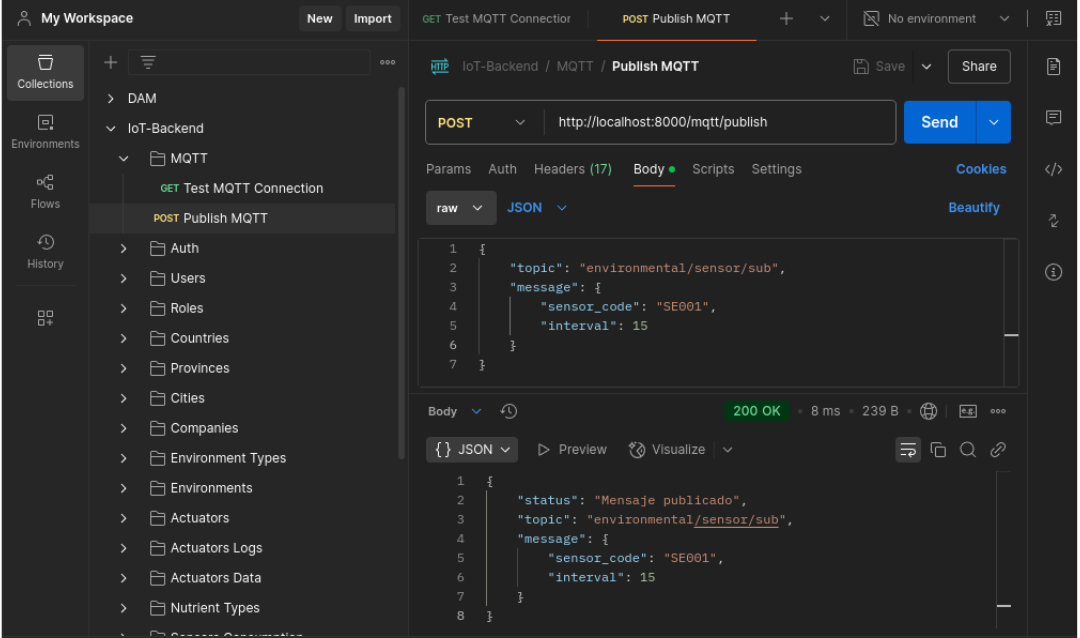
\includegraphics[width=.90\textwidth]{./Images/20.png}
    \caption{Pasos para verificar la conexión con el broker MQTT.}
    \label{fig:test_mqtt}
\end{figure}

La figura \ref{fig:publish_mqtt} muestra los pasos realizados para publicar un
mensaje en un tópico específico.

\begin{figure}[H]
    \centering
    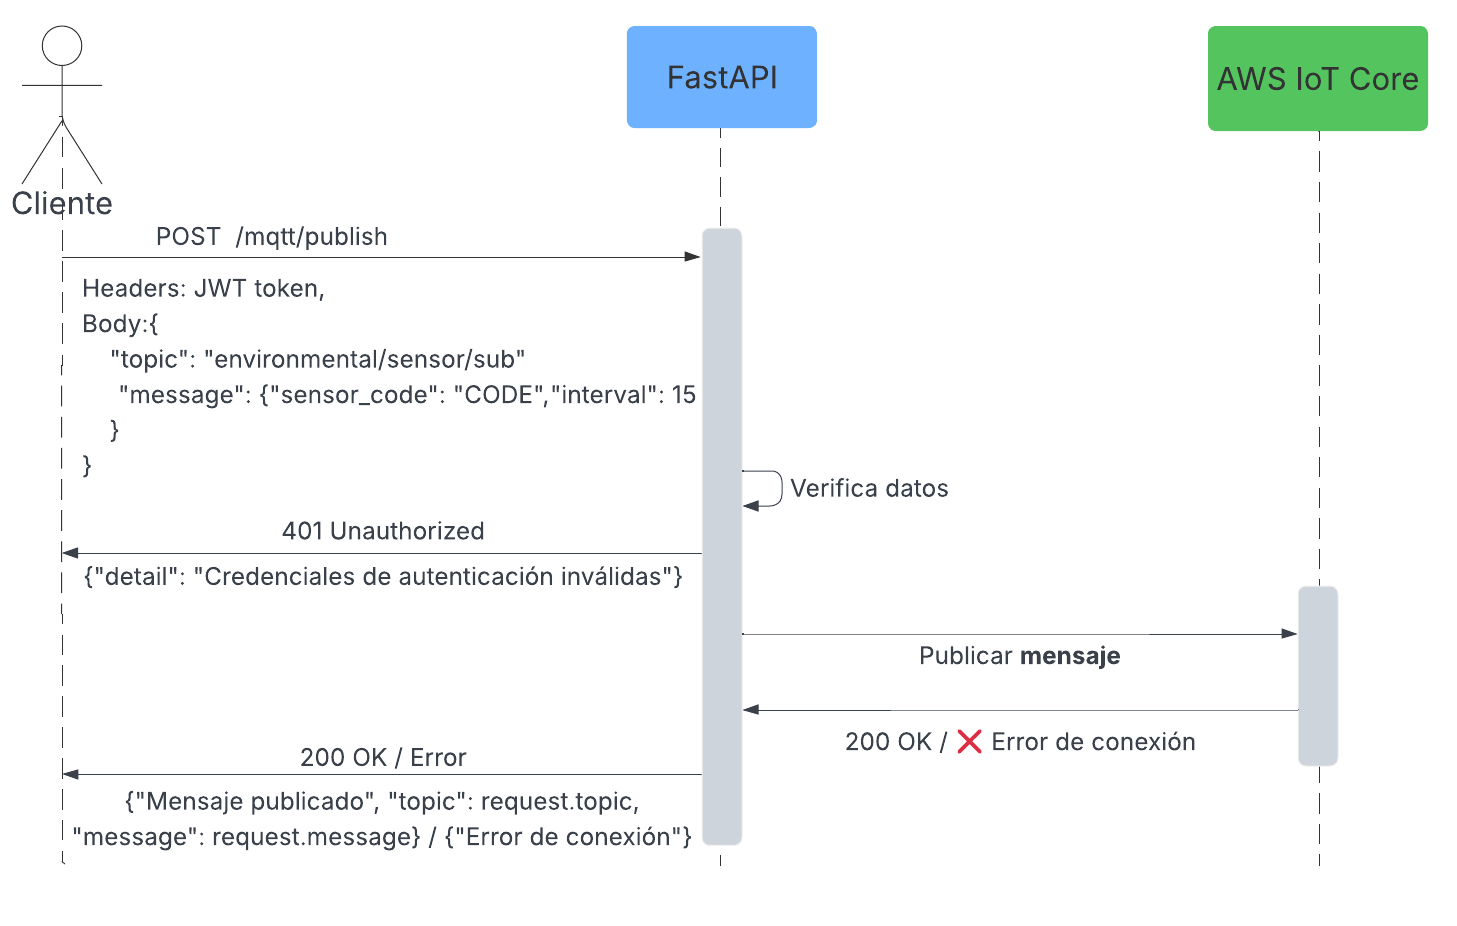
\includegraphics[width=.90\textwidth]{./Images/21.png}
    \caption{Pasos para publicar un mensaje en un tópico específico.}
    \label{fig:publish_mqtt}
\end{figure}

\subsubsection{Comunicación con MQTT en FastAPI}

Además de las rutas anteriores, en FastAPI se implementaron métodos para
suscribirse a los tópicos, recibir mensajes de los nodos y publicar en los
tópicos correspondientes.

Al iniciarse el servidor, el cliente MQTT establece la conexión con el broker y
se suscribe a los tópicos definidos. Los mensajes recibidos son procesados,
almacenados en MongoDB y enviados al frontend mediante WebSocket, lo que
permite actualizar la interfaz en tiempo real. Este cliente, que maneja la
conexión, publicación y suscripción, se inicializa junto con FastAPI para
asegurar una comunicación eficiente.

La figura \ref{fig:cliente_mqtt} describe la secuencia de acciones que permite
a la aplicación FastAPI conectarse al broker MQTT y suscribirse a los tópicos
requeridos.

\begin{figure}[H]
    \centering
    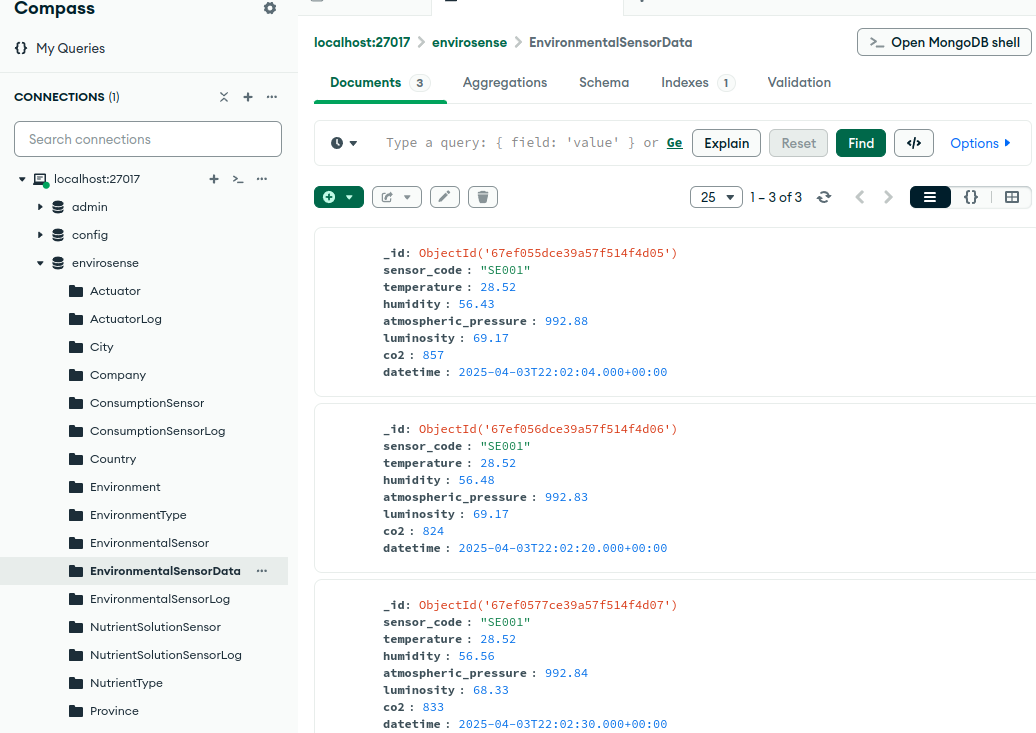
\includegraphics[width=.75\textwidth]{./Images/22.png}
    \caption{Pasos para la conexión del cliente MQTT.}
    \label{fig:cliente_mqtt}
\end{figure}

\subsection{Implementación de WebSocket}

La comunicación en tiempo real se implementó mediante el módulo
\texttt{websockets} de FastAPI, con una ruta específica para que los clientes
se conecten y reciban datos actualizados de sensores y actuadores. La conexión
permanece activa mientras sea válida, y se cierra en caso de error o falta de
autorización.

El cliente debe enviar un token válido por \texttt{Authorization}. Si es
válido, el servidor acepta la conexión y la gestiona a través de la clase
\texttt{WebSocketManager}.

Esta clase administra las conexiones activas, clientes y el envío de datos en
tiempo real. Además, mantiene un caché con los últimos valores por tipo de
sensor para optimizar el rendimiento. Al recibir nuevos datos, el servidor
actualiza el caché y los transmite a todos los clientes conectados.

La figura \ref{fig:websocket} ilustra el proceso de conexión.

\begin{figure}[H]
    \centering
    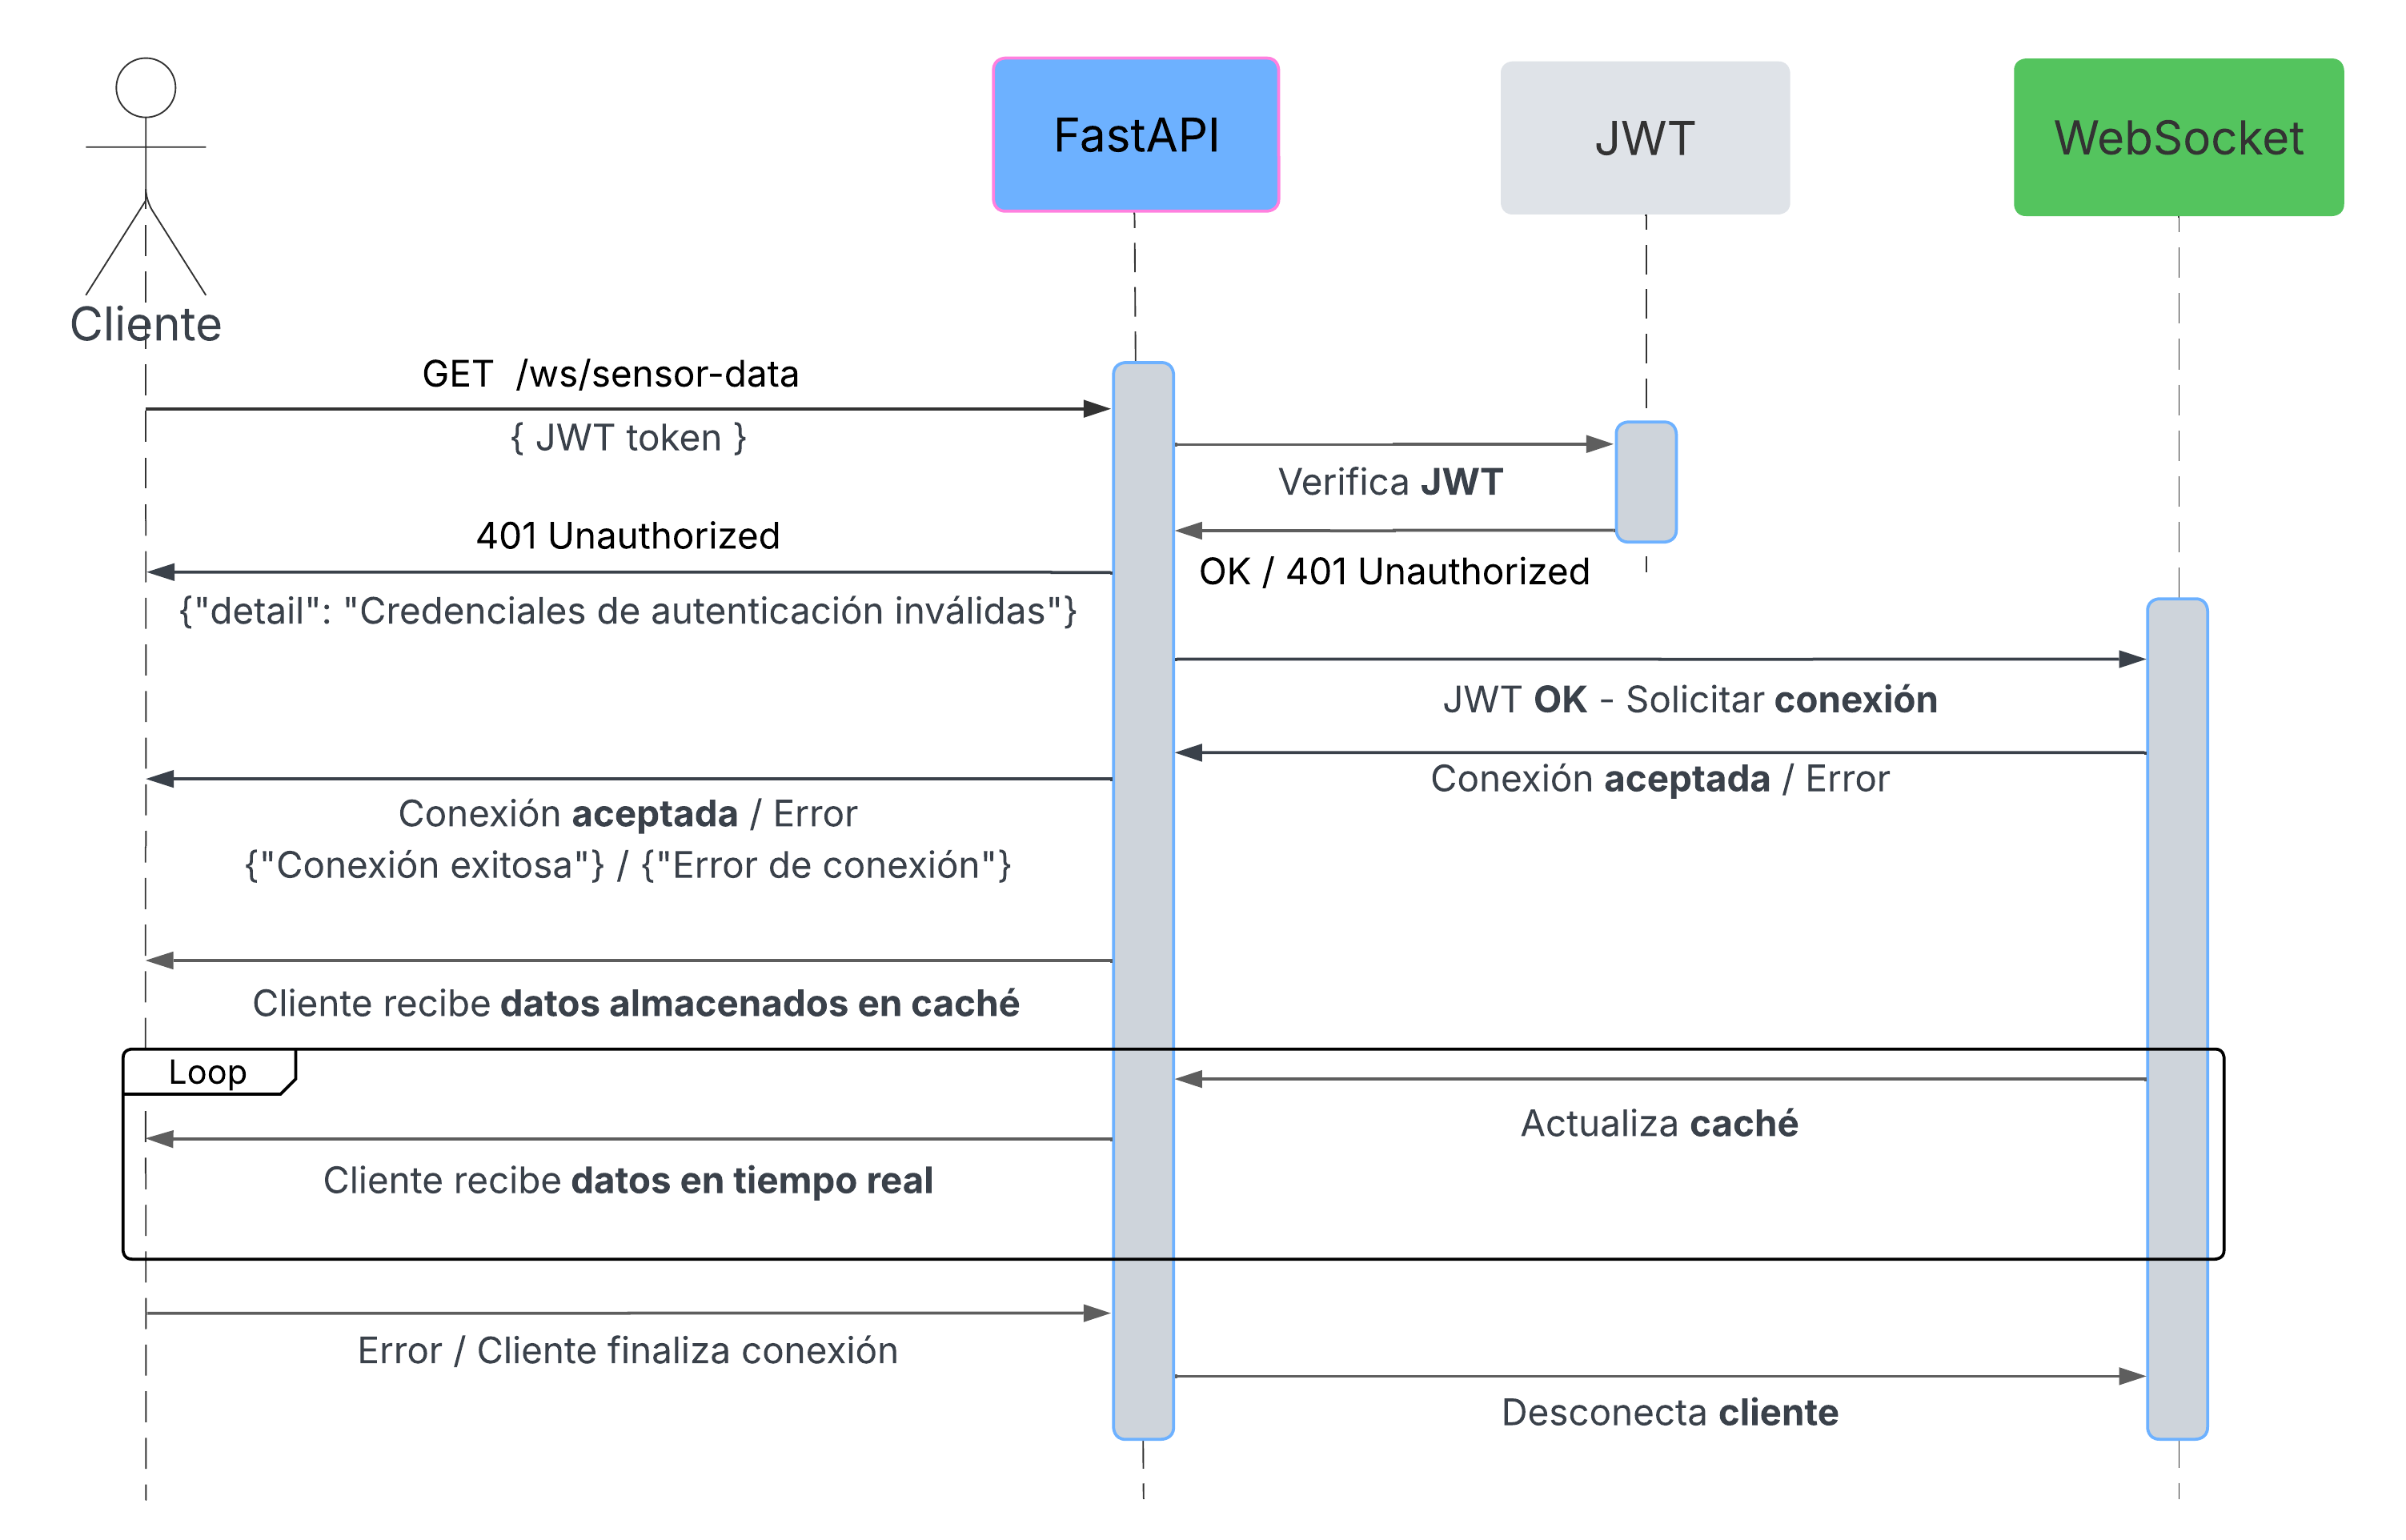
\includegraphics[width=.90\textwidth]{./Images/23.png}
    \caption{Pasos para establecer la conexión WebSocket.}
    \label{fig:websocket}
\end{figure}

%----------------------------------------------------------------------------------------
%	SECTION 5
%----------------------------------------------------------------------------------------
\section{Desarrollo del frontend}

En esta sección se describe el diseño y desarrollo de la interfaz de usuario,
enfocada en la visualización de datos en tiempo real y la gestión de
dispositivos a través de una aplicación web.

\subsection{Tecnologías utilizadas}

Como se mencionó anteriormente, el frontend se desarrolló a través de la
biblioteca React \cite{React}. Para los estilos y la disposición visual se
utilizó la biblioteca React Bootstrap \cite{ReactBootstrap}. Para los iconos de
la interfaz se utilizó Bootstrap Icons \cite{BootstrapIcons}, que proporciona
una amplia variedad de iconos gratuitos personalizables y fáciles de usar.

La comunicación con el servidor se implementó mediante la biblioteca Axios
\cite{Axios} para realizar solicitudes HTTP, mientras que la recepción de datos
en tiempo real se logró con la implementación de un WebSocket nativo, a través
de un \texttt{hook} personalizado desarrollado en React.

La gestión del estado de autenticación y control de sesiones se implementó con
Redux Toolkit \cite{ReduxToolkit} y la navegación entre páginas se gestionó a
través de la biblioteca React Router \cite{ReactRouter}.

Para la visualización de los gráficos, se empleó la biblioteca Recharts
\cite{Recharts}, mientras que para la representación de tablas se utilizó la
biblioteca React Data Table Component \cite{ReactDataTable}.

\subsection{Arquitectura de la interfaz}

La aplicación se estructuró en torno a un componente principal de
\texttt{layout}, que organiza la navegación mediante un \texttt{sidebar}
lateral y un \texttt{navbar} superior.

Cada sección de la interfaz de usuario corresponde a un módulo de funcionalidad
específica (como visualización en tiempo real, reportes, configuración de
ambientes, dispositivos, parámetros y administración de usuarios), que son
renderizados dinámicamente en función de la ruta activa.

\subsection{Componentes principales de la interfaz de usuario}

A continuación, se presenta el detalle de los principales componentes
desarrollados para la construcción de la interfaz.

\subsubsection{Gestión de autenticación}

La autenticación se implementó mediante un \texttt{hook} denominado
\texttt{useAuthStore}, basado en Redux Toolkit. Este módulo gestiona el inicio
de sesión, la validación del token y el cierre de sesión de los usuarios, para
asegurar el acceso restringido a las funcionalidades de la plataforma.

Al iniciar sesión, se almacena el token en el \texttt{localStorage} del
navegador, lo que permite mantener la sesión activa y acceder a las
funcionalidades de la aplicación. El token se envía en cada solicitud a la API
para autenticar al usuario y garantizar la seguridad de la comunicación.

La figura \ref{fig:login_sistema} muestra la pantalla de inicio de sesión,
donde los usuarios ingresan sus credenciales para acceder a la aplicación web.

\begin{figure}[H]
    \centering
    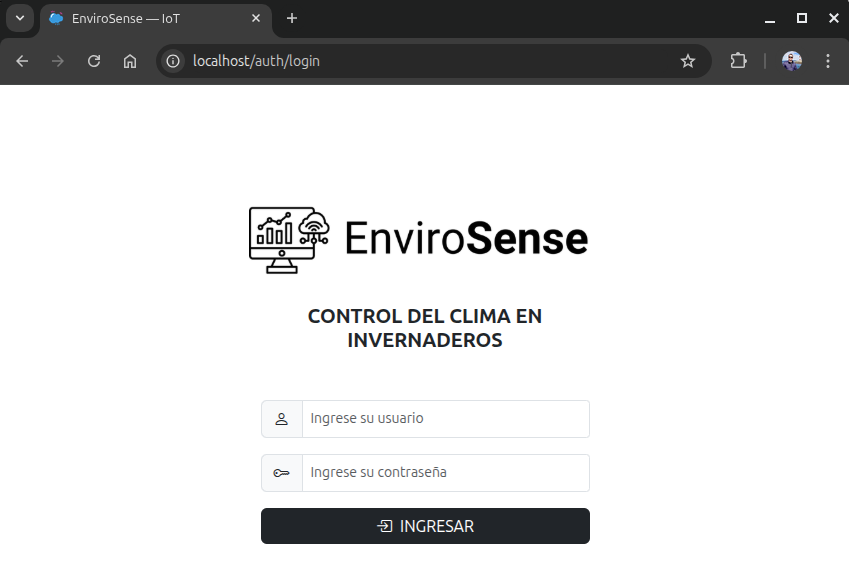
\includegraphics[width=0.80\textwidth]{./Images/24_login.png}
    \caption{Pantalla de inicio de sesión.}
    \label{fig:login_sistema}
\end{figure}

\subsubsection{Layout}

El componente \texttt{layout} organiza la estructura general de la aplicación e
incluye:
\begin{itemize}
    \item \texttt{Sidebar}: componente que muestra el menú lateral, con opciones de navegación
          entre los distintos módulos.
    \item \texttt{Navbar}: barra superior que permite colapsar o expandir el menú lateral y
          contiene el botón de cierre de sesión.
\end{itemize}

La figura \ref{fig:layout} muestra la pantalla principal de la aplicación,
donde se puede observar la barra de navegación superior y el menú lateral desde
el rol \texttt{admin}.

\begin{figure}[H]
    \centering
    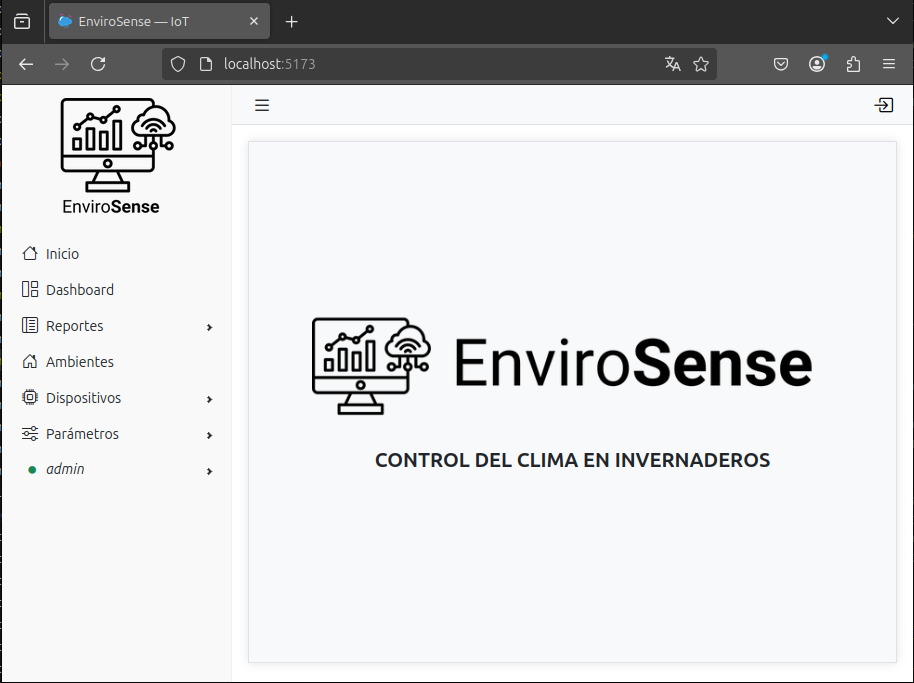
\includegraphics[width=0.90\textwidth]{./Images/25_layout.png}
    \caption{Pantalla principal de la aplicación web.}
    \label{fig:layout}
\end{figure}

Además, esta pantalla permite visualizar los módulos disponibles en la
aplicación, como dashboard, reportes, ambientes, dispositivos, parámetros y
panel de usuario.

\subsubsection{Arquitectura de navegación y control de acceso}

La aplicación implementa un sistema de navegación que gestiona dinámicamente
las rutas públicas y privadas mediante la biblioteca React Router. Utiliza los
componentes \texttt{Routes} para definir la estructura de navegación y
\texttt{Outlet} para renderizar sub-rutas.

Además, se implementa un flujo de acceso controlado por:

% \begin{itemize}
%     \item Rutas públicas: accesibles sin autenticación, como la página de inicio de
%           sesión.
%     \item Rutas privadas: requieren autenticación y autorización, como el acceso a los
%           módulos de la aplicación.
%     \item Rutas restringidas: accesibles solo para usuarios con los permisos adecuados,
%           como reportes, la gestión de usuarios, ambientes, y dispositivos.
% \end{itemize}

\begin{itemize}
    \item Rutas públicas: accesibles sin autenticación, como la página de inicio de
          sesión.
    \item Rutas privadas: requieren autenticación, destinadas a usuarios registrados que
          acceden a funcionalidades generales de la aplicación.
    \item Rutas restringidas: requieren autenticación y permisos específicos, habilitadas
          solo para ciertos roles (como administradores), por ejemplo para acceder a
          gestión de usuarios, ambientes y dispositivos.
\end{itemize}

Este esquema garantiza que cada usuario solo pueda acceder a las
funcionalidades habilitadas según sus permisos. Por ejemplo, como se muestra en
la figura \ref{fig:navegacion}, el usuario \texttt{martin}, con el rol de
usuario estándar, tiene acceso únicamente al dashboard, a los reportes y a su
panel de usuario, donde puede consultar su información personal.

\begin{figure}[H]
    \centering
    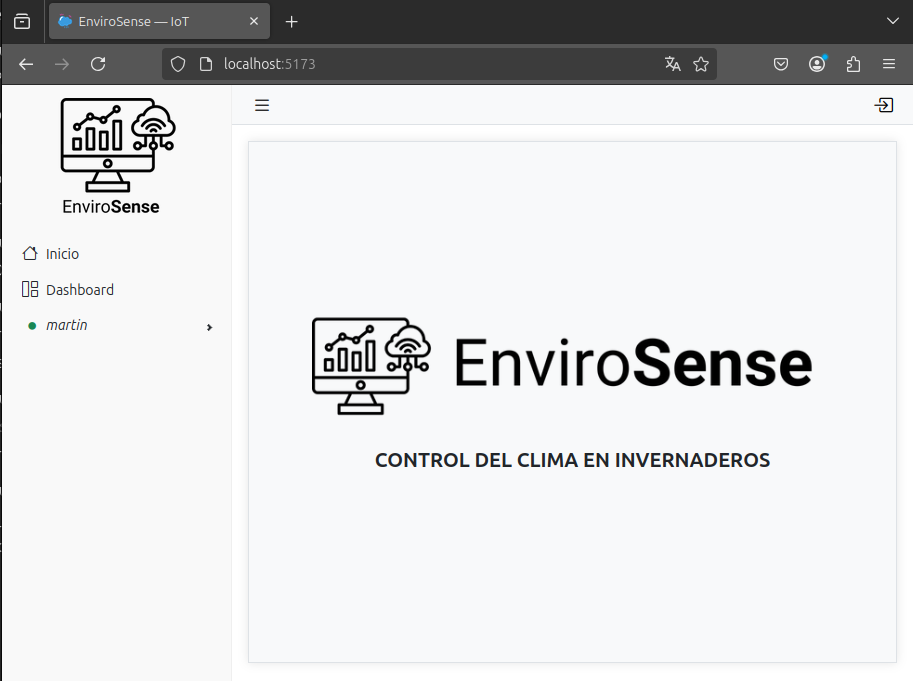
\includegraphics[width=0.90\textwidth]{./Images/26_navegacion.png}
    \caption{Interfaz de navegación según permisos de usuario estándar.}
    \label{fig:navegacion}
\end{figure}

\subsection{Visualización de datos en tiempo real}

Se desarrolló una página que permite visualizar en tiempo real los datos
recopilados por los sensores y el estado de los actuadores de un ambiente
específico. La información se actualiza automáticamente mediante el uso de
WebSocket a medida que se reciben nuevos datos.

La figura \ref{fig:dashboard_sistema} ilustra el dashboard de la aplicación,
donde se pueden observar los datos de los sensores y actuadores en tiempo real
de un ambiente específico.

\begin{figure}[H]
    \centering
    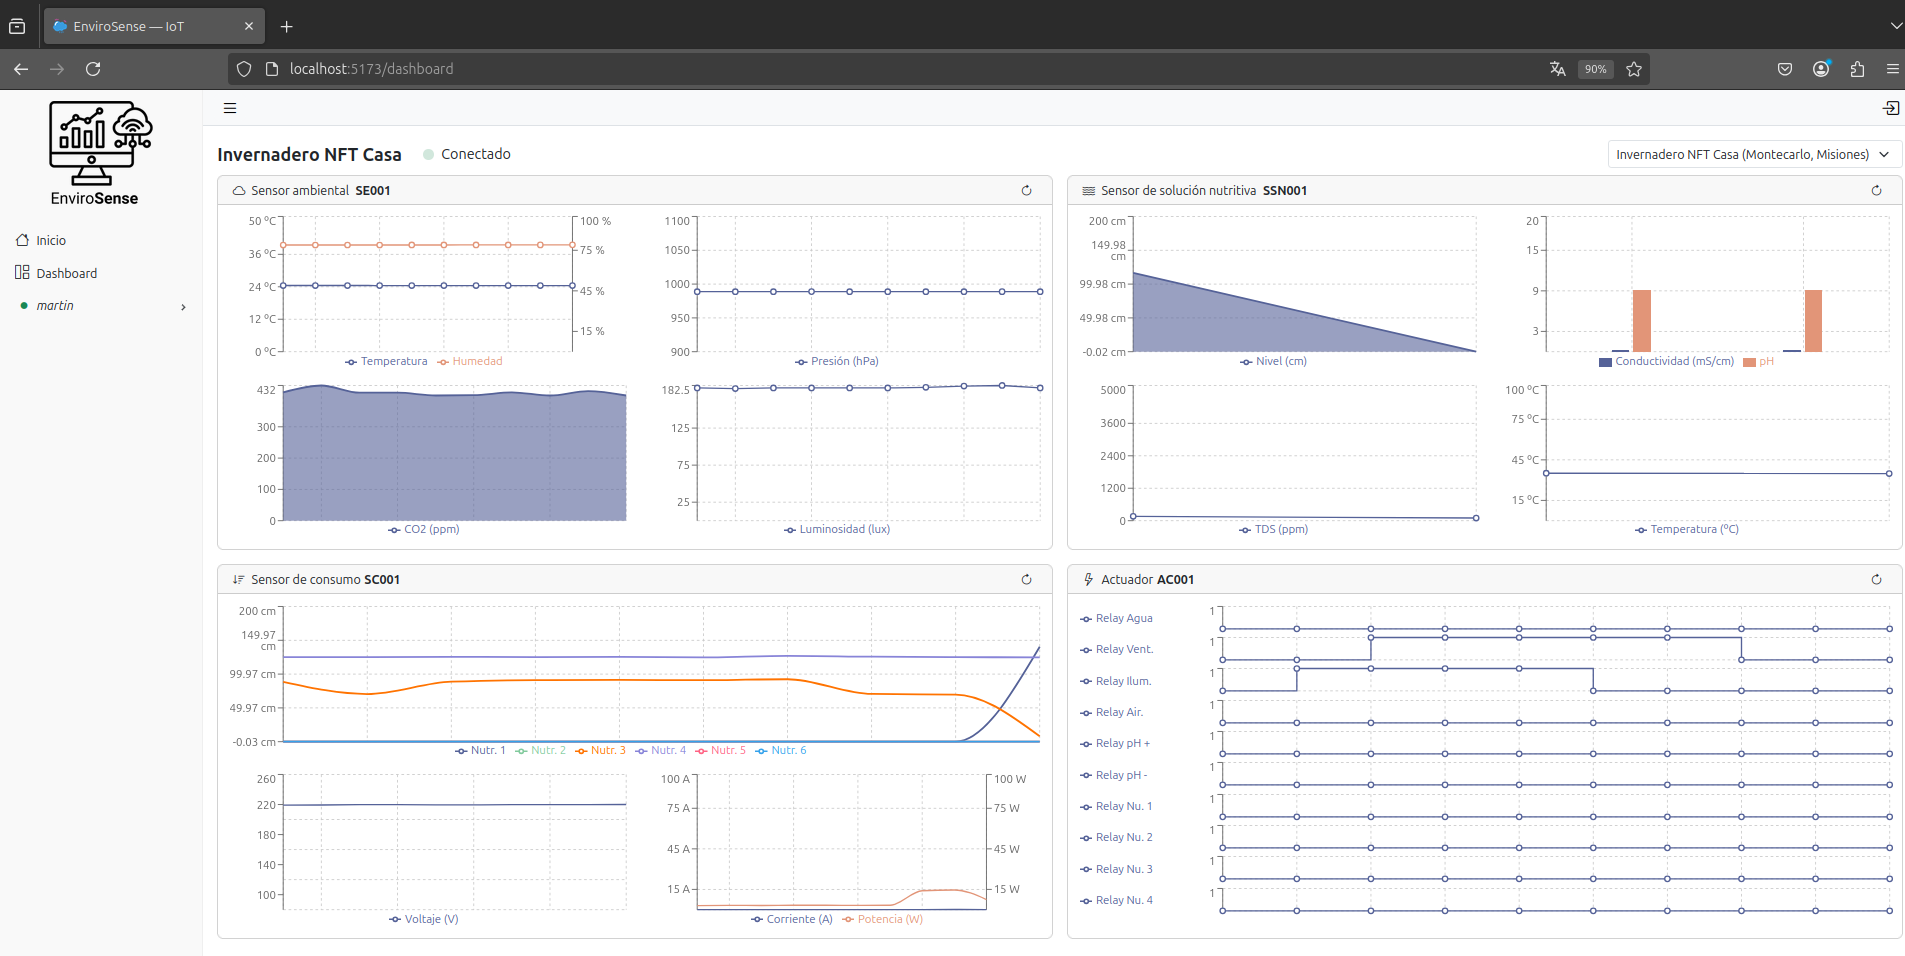
\includegraphics[width=\textwidth]{./Images/27_dashboard.png}
    \caption{Visualización de datos en tiempo real.}
    \label{fig:dashboard_sistema}
\end{figure}

\subsection{Reportes de datos históricos}

Se desarrollaron un conjunto de reportes que permiten visualizar los datos
históricos de los sensores y actuadores. Los diferentes tipos de reportes están
organizados en módulos independientes.

Cada reporte permite:
\begin{itemize}
    \item Filtrar los datos por dispositivo, rango de fechas y nivel de agregación
          temporal.
          \begin{itemize}
              \item Actuadores: el reporte permite visualizar la cantidad de veces que se activó y
                    el tiempo total de activación de cada canal del actuador.
              \item Sensores: el reporte permite visualizar el promedio de los datos recopilados
                    por cada sensor.
          \end{itemize}
    \item Alternar entre una vista tabular y una vista gráfica.
    \item Paginación de resultados en la vista tabular, para mejorar la navegación cuando
          hay grandes volúmenes de datos.
\end{itemize}

Los reportes obtienen la información procesada desde la API del backend, lo que
garantiza que los datos mostrados estén siempre actualizados.

La figura \ref{fig:reportes_tabla_consumos} presenta la pantalla de reportes,
donde se visualiza la tabla con los datos históricos de un sensor de consumos.

\begin{figure}[H]
    \centering
    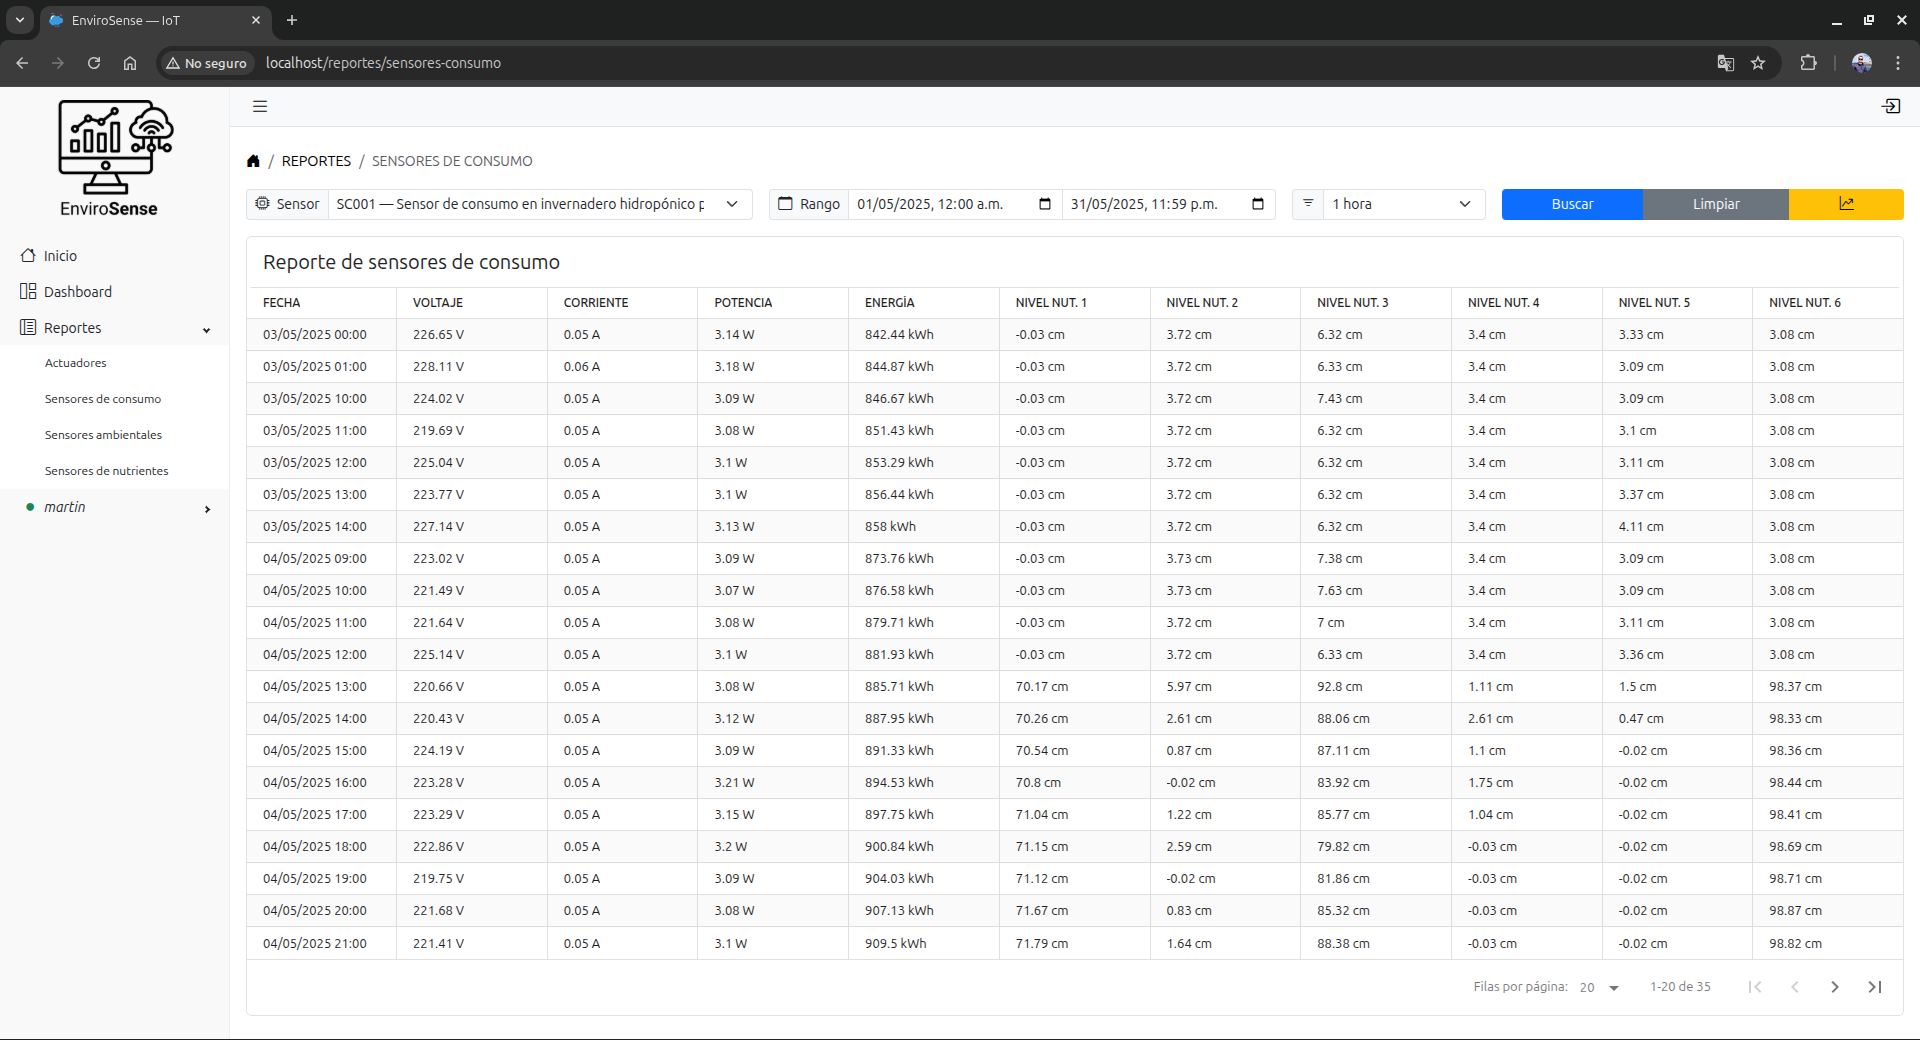
\includegraphics[width=\textwidth]{./Images/28_reportes_1.png}
    \caption{Pantalla de visualización tabular de consumos registrados.}
    \label{fig:reportes_tabla_consumos}
\end{figure}

La figura \ref{fig:reportes_graficos_consumos} muestra la pantalla de reportes,
donde se exhiben los gráficos con los datos históricos de un sensor de
consumos.

\begin{figure}[H]
    \centering
    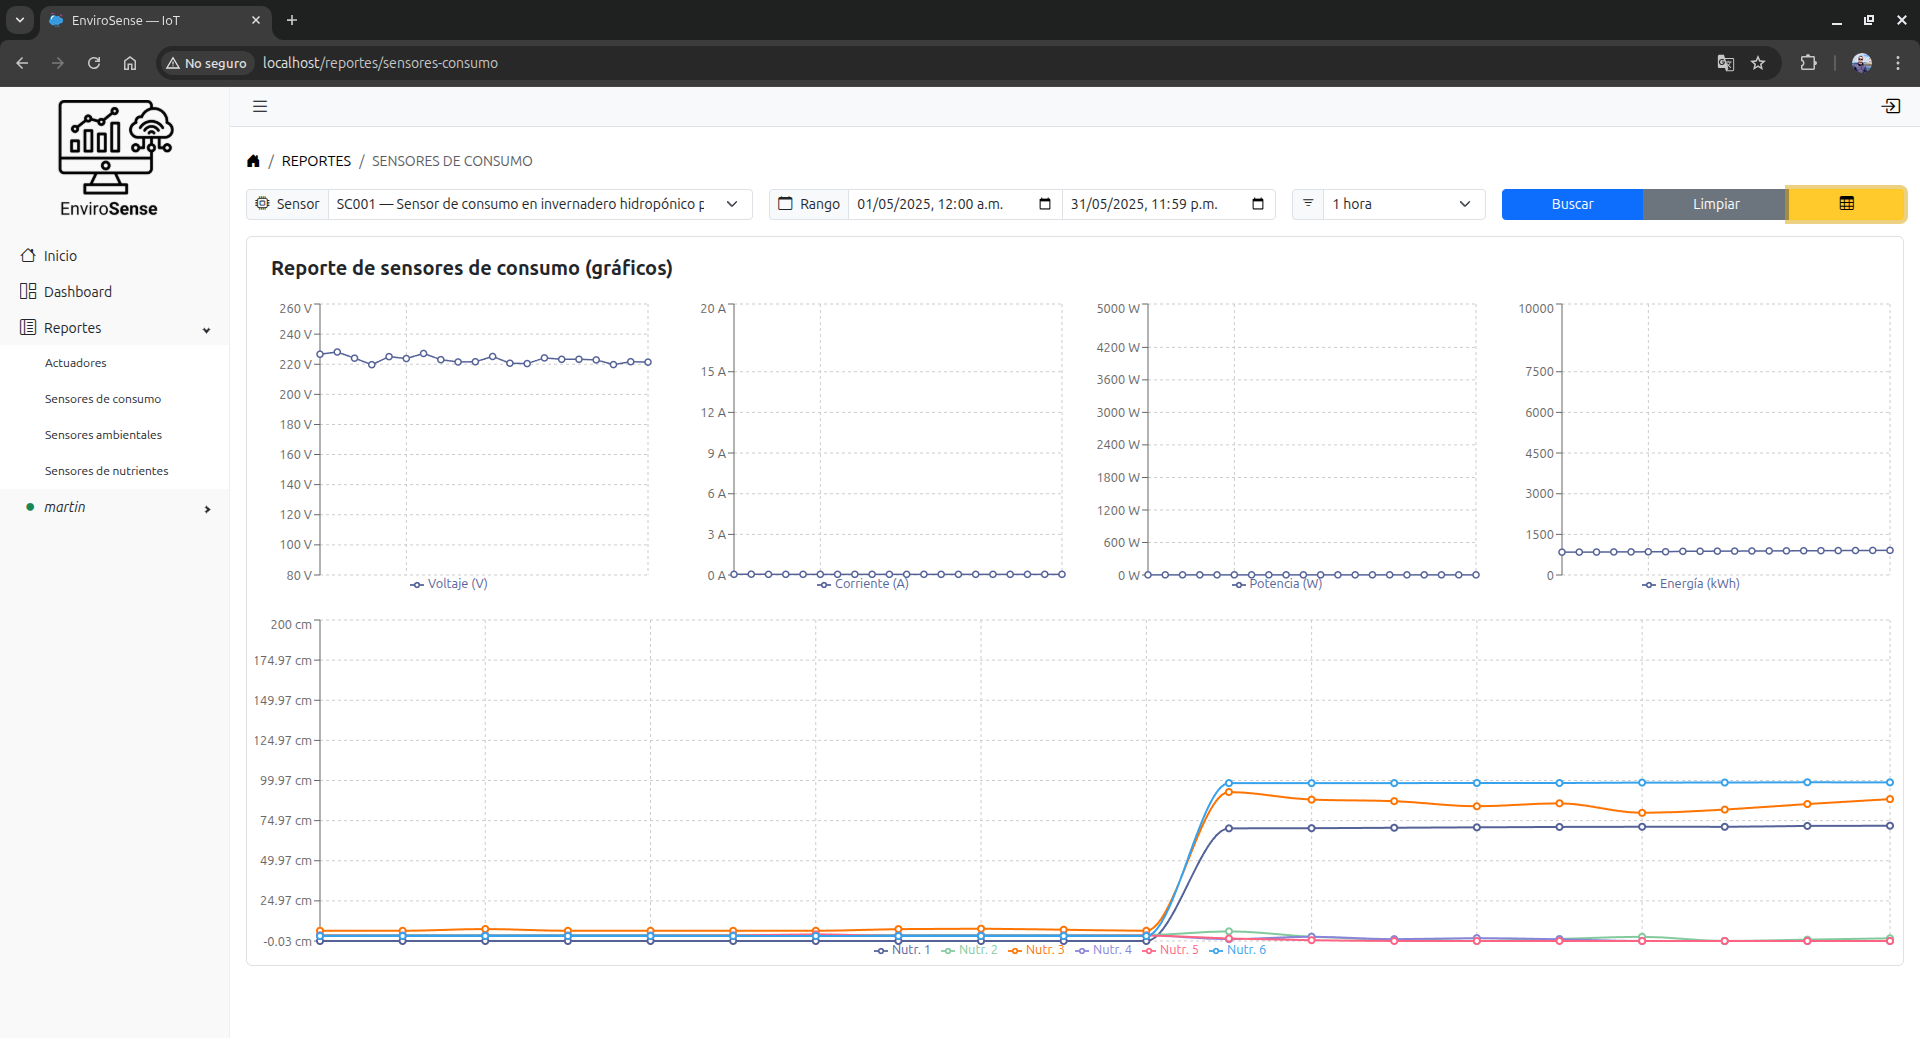
\includegraphics[width=\textwidth]{./Images/28_reportes_2.png}
    \caption{Pantalla de visualización de gráficos de consumos registrados.}
    \label{fig:reportes_graficos_consumos}
\end{figure}

La figura \ref{fig:reportes_tabla_actuadores} muestra la pantalla de reportes,
donde se puede observar la tabla con los datos históricos de un actuador.

\begin{figure}[H]
    \centering
    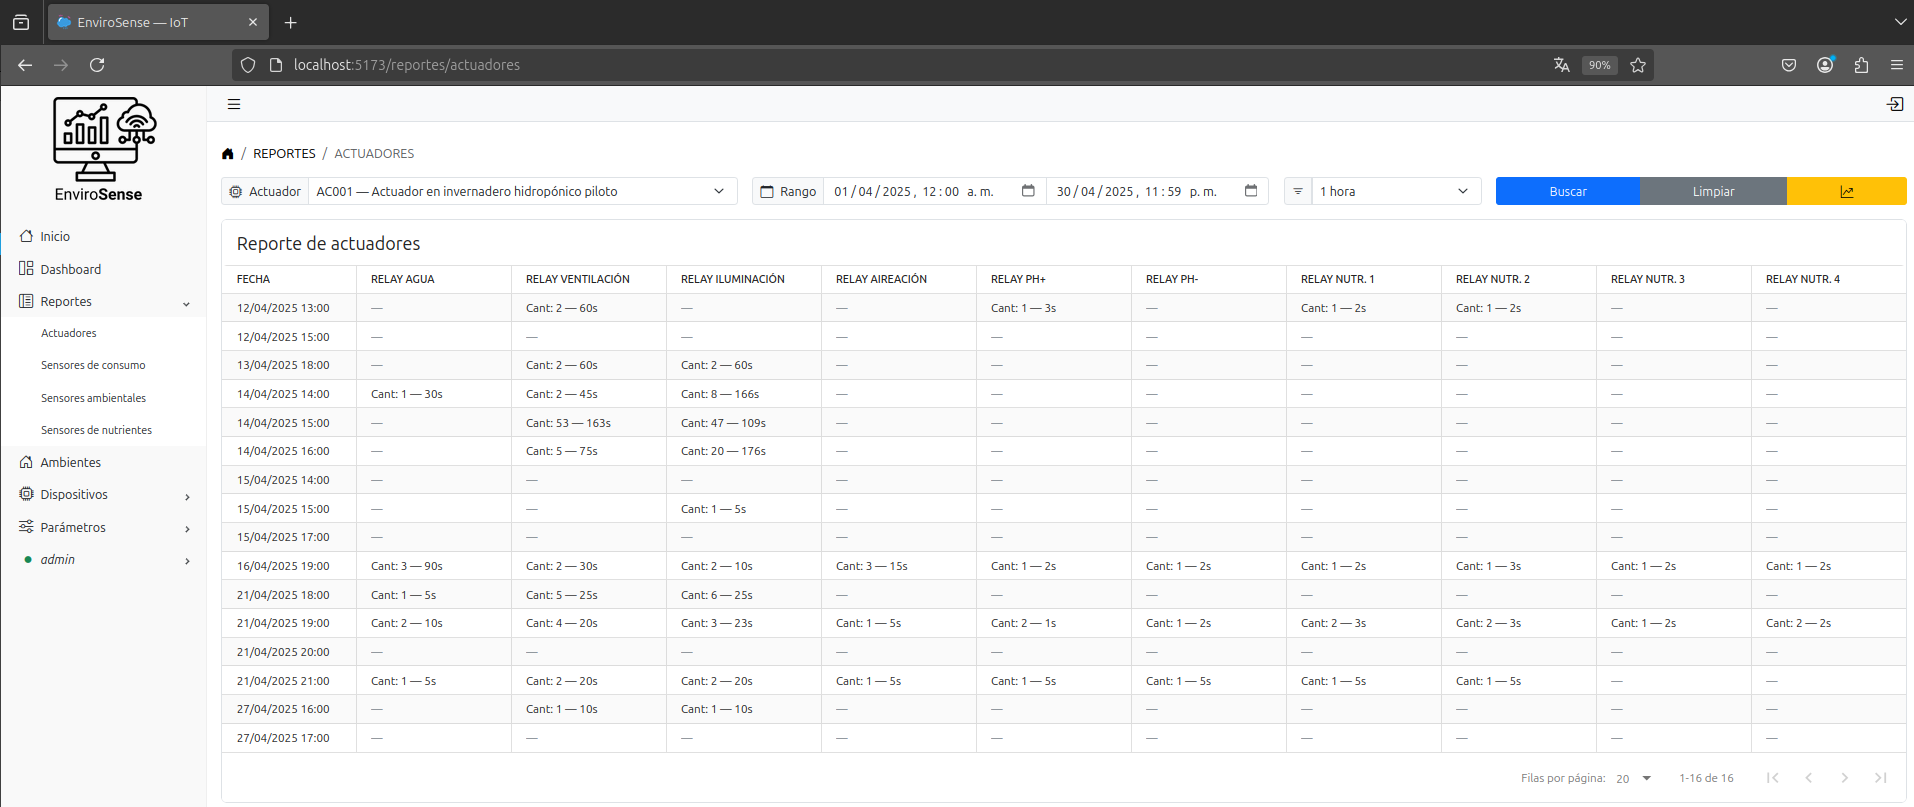
\includegraphics[width=\textwidth]{./Images/28_reportes_3.png}
    \caption{Pantalla de visualización tabular de actuadores.}
    \label{fig:reportes_tabla_actuadores}
\end{figure}

Finalmente, en la figura \ref{fig:dashboard_celular} se observa la interfaz de
la aplicación web en un dispositivo móvil, específicamente la pantalla de
visualización de datos en tiempo real. La interfaz se adapta de forma
automática a diferentes tamaños de pantalla, lo que permite una experiencia de
usuario optimizada tanto en teléfonos móviles como en tablets.

\begin{figure}[H]
    \centering
    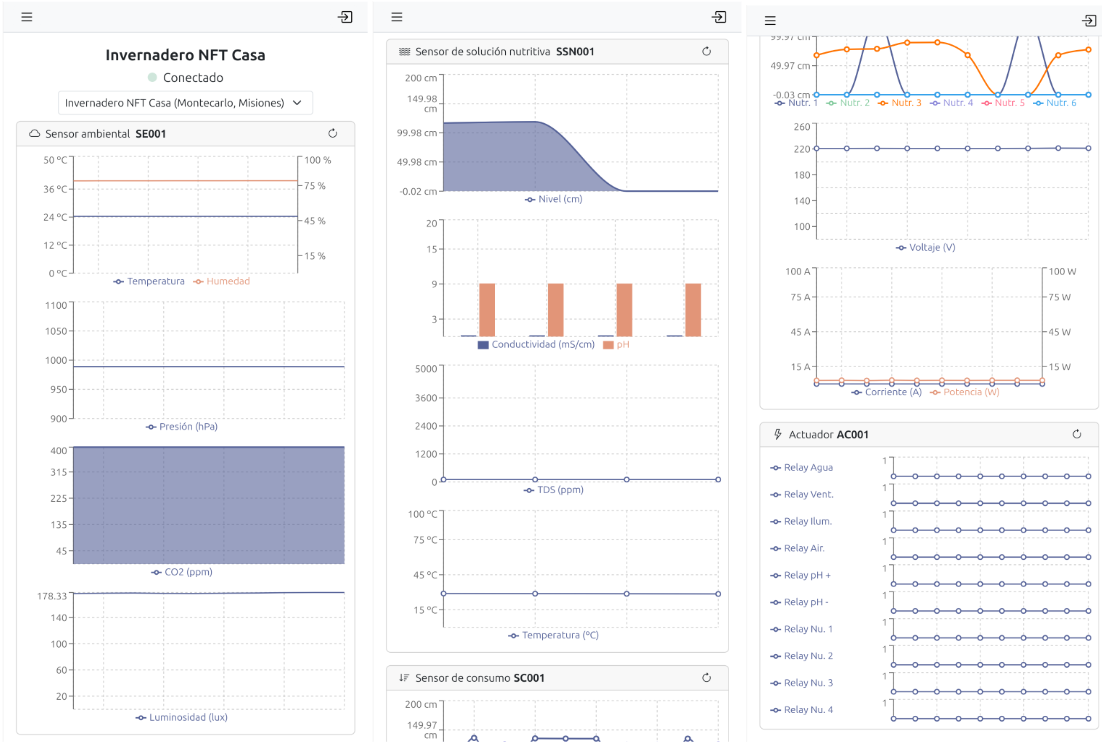
\includegraphics[width=\textwidth]{./Images/29_dashboard_celular.png}
    \caption{Visualización de datos en tiempo real desde un dispositivo móvil.}
    \label{fig:dashboard_celular}
\end{figure}

%----------------------------------------------------------------------------------------
%	SECTION 6
%----------------------------------------------------------------------------------------
\section{Desarrollo del firmware de los dispositivos IoT}

% Esta sección presenta el desarrollo del firmware implementado en MicroPython
% para los nodos del sistema. Se describe la arquitectura general del software
% embebido y la estructura del código fuente.

Esta sección presenta el desarrollo de los distintos firmwares implementados en
MicroPython para los diferentes tipos de nodos del sistema. Se describe la
arquitectura general del software embebido y la estructura del código fuente.

\subsection{Arquitectura general del firmware}

Todos los nodos comparten una arquitectura de firmware similar, diseñada para
realizar:

\begin{itemize}
    \item Adquisición de datos: lectura de sensores y actuadores.
    \item Control de actuadores: gestión de dispositivos conectados.
    \item Comunicación inalámbrica: conexión a la red Wi-Fi y broker MQTT.
    \item Gestión de eventos: manejo de interrupciones y temporizadores.
    \item Interacción con el broker MQTT: publicación y suscripción a tópicos.
\end{itemize}

% ----------------------------------------------------------------------------------------

\subsection{Estructura del código}

Para el desarrollo de los nodos, se adoptó un esquema de organización que
facilitó la modularidad, la reutilización de código y la facilidad de
mantenimiento.

La estructura es la siguiente:

\begin{enumerate}
    \item Importación de bibliotecas: importación de módulos para sensores, Wi-Fi, MQTT,
          gestión del tiempo y otras funcionalidades.
    \item Configuración inicial: definición de variables y constantes (pines, parámetros
          de conexión, intervalos).
    \item Inicialización: configuración de periféricos del ESP32, inicialización de
          sensores/relés y manejo de errores.
    \item Funciones auxiliares: definición de funciones para la conexión Wi-Fi,
          sincronización NTP (del inglés, \textit{Network Time Protocol}) y carga de
          certificados TLS.
    \item Conexión MQTT: establecimiento de la conexión con el broker MQTT con
          certificados TLS.
    \item Callback de mensajes MQTT: función para procesar mensajes MQTT (configuración
          remota, acciones específicas).
    \item Función de lectura/control: implementación de la lógica para leer sensores o
          controlar actuadores.
    \item Bucle principal:
          \begin{enumerate}
              \item Verificación de la conexión Wi-Fi.
              \item Lectura de datos de los sensores o control de los actuadores.
              \item Envío de datos al broker MQTT.
              \item Recepción y procesamiento de mensajes MQTT.
              \item Gestión de errores y reinicio del sistema en caso de fallos.
          \end{enumerate}
\end{enumerate}

La figura \ref{fig:flujo_nodos} muestra el flujo general del firmware, desde la
inicialización hasta el bucle principal, con manejo de comandos MQTT y acciones
sobre sensores y actuadores.

\begin{figure}[H]
    \centering
    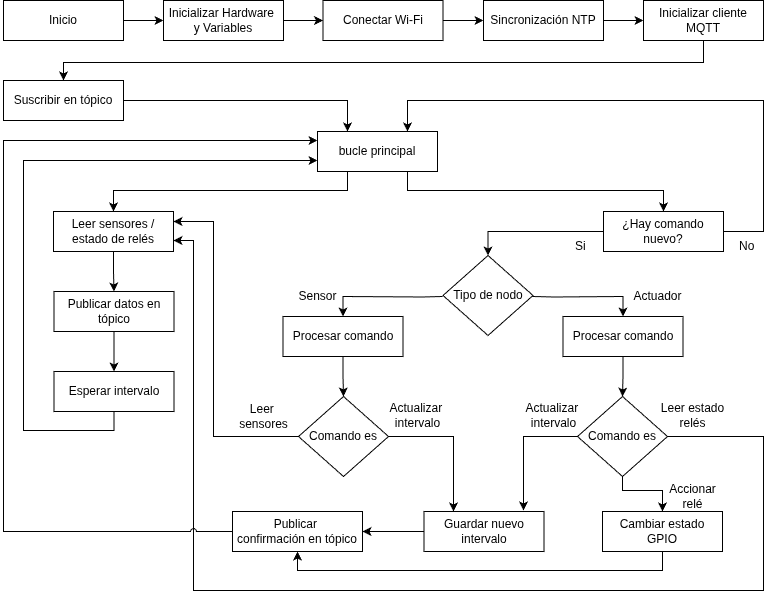
\includegraphics[width=0.96\textwidth]{./Images/30_flujo_ppal_nodos.png}
    \caption{Flujo de ejecución del código en los nodos.}
    \label{fig:flujo_nodos}
\end{figure}

% ----------------------------------------------------------------------------------------

\subsection{Gestión de la configuración}

La configuración de los parámetros operativos de cada nodo se almacenó en
archivos locales en el ESP32, lo que garantizó la persistencia de la
configuración incluso después de reinicios.

A continuación, se detallan los archivos de configuración utilizados en los
nodos:

\subsubsection{Archivo de configuración}

El archivo \texttt{config.py} contiene constantes y variables de configuración
específicas de cada nodo. Incluye:
\begin{itemize}
    \item Códigos de identificación: código único que permite identificar de manera
          unívoca a cada dispositivo.
    \item Tópicos MQTT: define los tópicos utilizados para la publicación de datos y la
          recepción de comandos. Cada nodo cuenta con un tópico de envío y otro de
          recepción.
    \item Parámetros de conexión AWS IoT Core: identificador del cliente y el endpoint
          del broker MQTT.
\end{itemize}

\subsubsection{Archivo de configuración del intervalo}

El archivo \texttt{interval.conf} almacena el intervalo de muestreo de sensores
y actuadores. Al iniciar el dispositivo, se intenta leer este valor; si el
archivo no existe o está corrupto, se usa un valor por defecto (15 segundos).
El intervalo puede actualizarse remotamente mediante MQTT, se sobrescribe el
archivo para conservar la nueva configuración tras reinicios.

\subsubsection{Archivo de configuración Wi-Fi}

El archivo \texttt{wifi.dat} almacena los parámetros de conexión Wi-Fi (SSID y
contraseña), permite guardar múltiples configuraciones de red. Si el nodo no
logra conectarse, se inicia un servidor web para que el usuario seleccione el
SSID, ingrese la contraseña y defina la zona horaria. Al configurarse con
éxito, los datos se guardan en el archivo y el dispositivo se reinicia.

\subsubsection{Archivo de configuración de la zona horaria}

La zona horaria se obtiene desde el archivo \texttt{timezone.conf} para
garantizar la marca de tiempo correcta. Esta funcionalidad se utiliza en los
nodos sensores y actuadores con el fin de incluir la hora local en los mensajes
enviados al broker MQTT. En caso de error en la lectura del archivo, se asigna
una zona horaria por defecto, en este caso, la de Argentina (\texttt{UTC-3}).

% ----------------------------------------------------------------------------------------

\subsection{Comunicación inalámbrica}

Los nodos desarrollados utilizan la comunicación Wi-Fi para conectarse a la red
local y enviar datos al broker MQTT a través de Internet.

A continuación, se describen las bibliotecas utilizadas para gestionar la
comunicación inalámbrica:

\subsubsection{Wi-Fi}

Para gestionar la conexión Wi-Fi, se empleó la biblioteca Wifi Manager
\cite{MicroPythonWifiManager}. Al iniciar, los nodos intentan conectarse a la
red configurada y realizan verificaciones periódicas para asegurar su
disponibilidad.

La biblioteca se modificó para adaptarla a los requerimientos del trabajo. Se
agregó la capacidad de almacenar datos de redes cuyo SSID contenga espacios en
blanco y se implementó un menú desplegable para la selección de la zona
horaria.

\subsubsection{MQTT}

Para desarrollar la comunicación MQTT, se utilizó la biblioteca
\texttt{umqtt.robust} de MicroPythonLib \cite{MicropythonLib}, que permitió
implementar un cliente MQTT en los nodos. Se estableció la conexión al broker
MQTT de AWS IoT Core mediante certificados TLS almacenados localmente en cada
dispositivo.

La figura \ref{fig:secuencia_mqtt} ilustra el flujo de comunicación
bidireccional entre los nodos, el broker MQTT de AWS IoT Core y el backend en
FastAPI, mediante conexiones TLS y tópicos específicos. Los nodos envían datos
y reciben comandos, mientras que el backend centraliza la gestión de las
comunicaciones.

\begin{figure}[H]
    \centering
    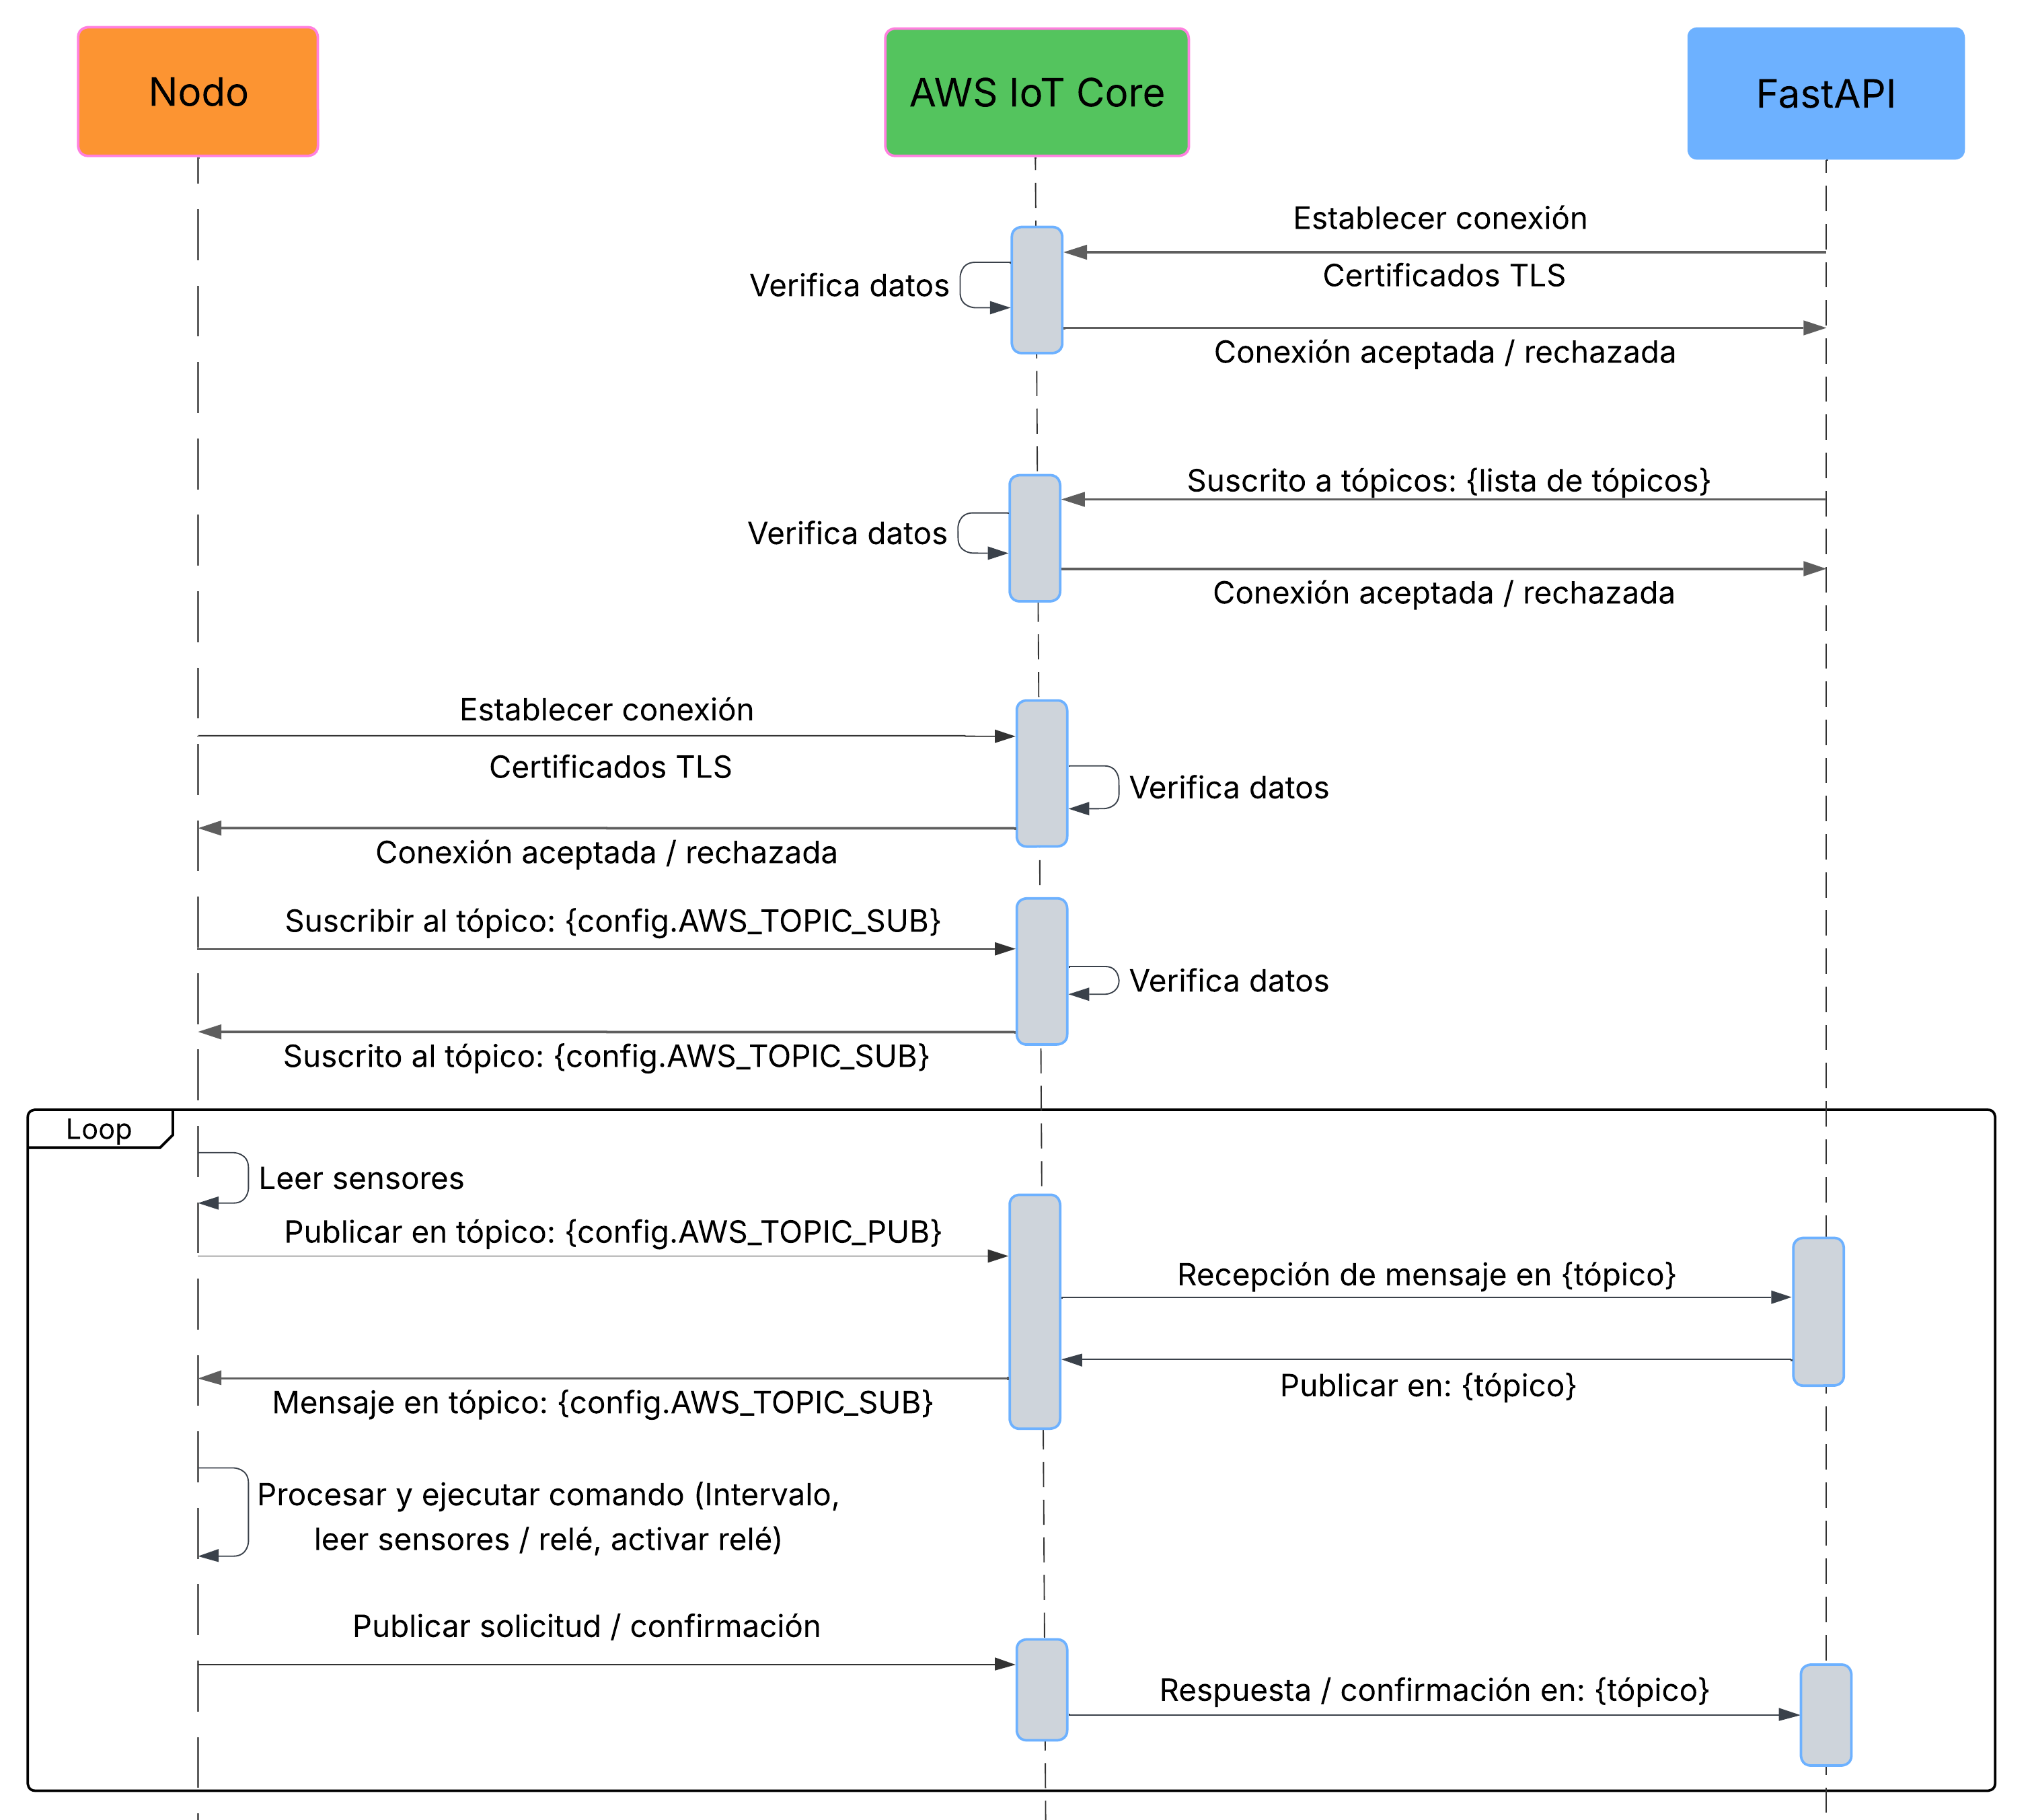
\includegraphics[width=0.82\textwidth]{./Images/31_secuencia_mqtt.png}
    \caption{Flujo de comunicación entre nodos y broker MQTT.}
    \label{fig:secuencia_mqtt}
\end{figure}

\subsubsection{Comunicación y formato de mensajes}

Los datos de sensores, actuadores y los comandos de control se transmiten
mediante MQTT, en formato JSON, y se publican en los tópicos definidos en el
archivo \texttt{config.py}. Se implementó un esquema estandarizado para
simplificar el procesamiento tanto en los nodos como en el backend.

% ----------------------------------------------------------------------------------------

\subsection{Gestión de tareas y concurrencia}

La ejecución concurrente de tareas en MicroPython se logró mediante la
implementación de:

\begin{itemize}
    \item Un bucle principal para tareas como:
          \begin{itemize}
              \item Conexión Wi-Fi.
              \item Procesamiento de mensajes MQTT.
              \item Lectura de datos de sensores.
          \end{itemize}
    \item Temporizadores hardware (\texttt{Timers}) del ESP32 para:
          \begin{itemize}
              \item Ejecutar acciones periódicas (por ejemplo: control de actuadores).
              \item Procesar tareas en paralelo sin afectar el flujo principal.
          \end{itemize}
\end{itemize}

% ----------------------------------------------------------------------------------------

\subsection{Manejo de errores}

Se implementaron mecanismos en todo el firmware para garantizar la robustez y
confiabilidad de los nodos frente a posibles fallos. A continuación, se
detallan las principales estrategias implementadas para la gestión de errores:

\subsubsection{Manejo de excepciones}

Se utilizaron bloques \texttt{try-except} para capturar y manejar excepciones
durante la ejecución. De este modo, el programa puede continuar operativo
incluso ante errores como fallos en la lectura de sensores o problemas de
conexión a la red.

\subsubsection{Reintentos}

Para operaciones críticas, como la conexión Wi-Fi y la sincronización de la
hora con el servidor NTP, se implementaron mecanismos de reintento. Si una
operación falla, el programa intenta repetirla un número preestablecido de
veces antes de considerarla fallida.

\subsubsection{Logging}

Se implementaron mensajes de registro (\texttt{print}) para informar sobre el
estado del programa y los errores que se producen. Esto facilitó la depuración
y el mantenimiento del firmware.

\subsubsection{Optimización de recursos}

Se empleó la función \texttt{gc.collect()} para liberar memoria de forma
periódica y optimizar el rendimiento del sistema. Esta función se invoca, por
ejemplo, luego de la lectura de sensores o del envío de datos al broker MQTT.

\subsection{Resumen de nodos sensores y actuadores}

La tabla \ref{tab:nodos_iot} resume las funciones y descripción general del
firmware de los nodos sensores y actuadores, diseñados para adquirir datos del
entorno o controlar dispositivos.

\begin{table}[H]
    \centering
    \caption[Resumen de nodos]{Resumen de nodos: funciones y firmware.}
    % \begin{tabular}{l l l}
    \begin{tabular}{p{1.5cm}p{5.4cm}p{5.5cm}}
        \toprule
        \textbf{Nodo}                                     & \textbf{Funciones principales}                                  & \textbf{Descripción del firmware}               \\
        \midrule
        \multirow{7}{1.5cm}{Sensor ambiental}             & Medición de temperatura, humedad y presión (BME280).            & Comunicación I\textsuperscript{2}C para BME280. \\
                                                          & Medición del nivel de iluminación (BH1750).                     & UART para MH-Z19C.                              \\
                                                          & Medición de concentración de $CO_2$ (MH-Z19C).                  & Medición inicial de $CO_2$.                     \\
                                                          & Conexión Wi-Fi.                     Conexión broker MQTT.       & Envío de datos en JSON vía MQTT.                \\
                                                          & Configuración de intervalo.                                     & Sincronización NTP.                             \\
                                                          & Indicador LED.                                                  & Reconexión Wi-Fi automática.                    \\
        \midrule
        \multirow{6}{1.5cm}{Sensor de consumos}           & Medición de voltaje, corriente y potencia (PZEM-004T).          & Uso de UART para PZEM-004T.                     \\
                                                          & Medición de nivel de líquidos (HC-SR04).                        & GPIO para HC-SR04.                              \\
                                                          & Conexión Wi-Fi.                     Conexión broker MQTT.       & Envío de datos en formato JSON vía MQTT.        \\
                                                          & Configuración de intervalo.                                     & Sincronización NTP.                             \\
                                                          & Indicador LED.                                                  & Reconexión Wi-Fi automática.                    \\
        \midrule
        \multirow{7}{1.5cm}{Sensor de solución nutritiva} & Medición de temperatura (DS18B20).                              & Lectura OneWire para DS18B20.                   \\
                                                          & Medición de pH, CE y TDS.                                       & Medición de CE,TDS y pH.                        \\
                                                          & Medición de nivel de líquidos (HC-SR04).                        & Promedio de muestras.                           \\
                                                          & Conexión Wi-Fi.                     Conexión broker MQTT.       & Envío de datos en JSON vía MQTT.                \\
                                                          & Configuración de intervalo.                                     & Sincronización NTP.                             \\
                                                          & Indicador LED.                                                  & Reconexión Wi-Fi automática.                    \\
        \midrule
        \multirow{7}{1.5cm}{Actuador}                     & Control de relés para dispositivos (bombas, aireadores, luces). & Control de salidas GPIO.                        \\
                                                          & Ejecución simultánea de comandos.                               & Recepción de comandos MQTT.                     \\
                                                          & Conexión Wi-Fi.                     Conexión broker MQTT.       & Ejecución de temporizadores con Timers ESP32.   \\
                                                          & Configuración de intervalo.                                     & Manejo de estados de relés en JSON.             \\
                                                          & Indicador LED.                                                  & Sincronización NTP.                             \\
        \bottomrule
        \hline
    \end{tabular}
    \label{tab:nodos_iot}
\end{table}

\subsubsection{Herramientas de despliegue y monitoreo}

El despliegue del firmware en los nodos se realizó mediante el uso de PyMakr.
Esta herramienta permitió:

\begin{itemize}
    \item Transferir los archivos del firmware (como \texttt{main.py}, \texttt{config.py}
          y los certificados TLS) al sistema de archivos interno del ESP32.
    \item Establecer una conexión serial para monitorear logs en tiempo real durante la
          depuración.
\end{itemize}

Su integración con el entorno de desarrollo resultó fundamental para facilitar
tanto la implementación como la depuración del firmware en los nodos.

%----------------------------------------------------------------------------------------
%	SECTION 7
%----------------------------------------------------------------------------------------
\section{Despliegue del sistema}

En esta sección se describe el proceso de implementación y configuración del
sistema en un entorno de prueba basado en una instancia EC2 AWS. Se detalla la
instalación de los componentes, los pasos para realizar la clonación y
ejecución del sistema, así como la configuración del servicio para su
ejecución.

\subsection{Entorno de prueba}

\subsubsection{Creación de la instancia EC2}

El sistema fue desplegado en una instancia EC2 de AWS con las siguientes
características:

\begin{itemize}
    % \item Nombre: envirosense-app.
    \item Imagen de maquina de Amazon: Ubuntu Server 24.04 LTS (64-bit x86).
    \item Tipo de instancia: t2.micro (1 vCPU, 1 GB de RAM).
    \item Almacenamiento: 8 GB tipo gp3.
    \item Región: us-east-1.
    \item Grupo de seguridad: puertos abiertos para HTTP (80), HTTPS (443), SSH (22),
          WebSocket (8000) y acceso a la base de datos (27017).
\end{itemize}

El acceso a la instancia se realizó mediante SSH (del inglés, \textit{Secure
    Shell}). Para ello, se generó un par de claves RSA (Rivest, Shamir y Adleman) y
se descargó el archivo \texttt{envirosense-app-key.pem}, necesario para
establecer la conexión.

\subsubsection{Acceso remoto y configuración inicial}

Una vez lanzada la instancia, se accedió a la misma mediante SSH y se procedió
a actualizar los paquetes del sistema operativo.

A continuación, se instalaron las siguientes herramientas:
\begin{itemize}
    \item Docker: para los contenedores de la aplicación.
    \item Docker Compose: para la orquestación de los contenedores.
    \item DuckDNS \cite{DuckDNS}: para asociar nombre de dominio a la IP pública
          dinámica.
\end{itemize}

\subsection{Instalación de componentes del sistema}

\subsubsection{Docker y Docker Compose}

Como se mencionó en la sección \ref{sec:arquitecturaServidor}, se utilizó
Docker para generar tres contenedores:

\begin{itemize}
    \item Backend: contenedor con la imagen base \texttt{python} que ejecuta la API
          desarrollada en FastAPI.
    \item Frontend: contenedor que utiliza imágenes base de \texttt{node} y
          \texttt{nginx} para ejecutar un servidor HTTP con NGINX \cite{NGINX} y servir
          la aplicación web desarrollada en React.
    \item Base de datos: contenedor basado en la imagen oficial de \texttt{mongo}, que
          ejecuta una instancia de MongoDB para almacenar los datos de la aplicación.
\end{itemize}

Mediante el archivo \texttt{docker-compose.yml}, se definieron y orquestaron
los contenedores con Docker Compose. Se establecieron parámetros de
configuración para la comunicación entre contenedores, persistencia de datos,
variables de entorno, puertos y redes.

Los contenedores del backend y el frontend cuentan con sus respectivos
Dockerfile, donde se especificaron las instrucciones para construir las
imágenes de cada servicio. Estos archivos definen el entorno, dependencias y
comandos para ejecutar cada servicio.

\subsubsection{Cliente de actualización dinámica de DuckDNS}

Dado que se trata de un entorno de prueba, no fue necesario utilizar el
servicio de IP elástica de AWS para mantener una dirección fija. En su lugar,
se optó por emplear el servicio DuckDNS, que permite asociar un nombre de
dominio gratuito a la IP pública de la instancia EC2.

Se configuró un cliente de actualización, que se ejecuta en la instancia cada
cinco minutos para actualizar automáticamente la IP pública. Esto facilita el
acceso remoto al sistema sin necesidad de recordar una IP dinámica.

\subsubsection{Clonación del repositorio y preparación}

El código fuente del sistema fue clonado en la máquina virtual desde un
repositorio público de GitHub \cite{EnviroSenseIoT}. Dentro del directorio del
sistema, se preparó un archivo de variables de entorno (\texttt{.env}) que
contiene información sensible y parámetros de configuración del sistema. Este
archivo no forma parte del repositorio, por lo que fue creado manualmente en la
instancia. En él se definieron las siguientes variables necesarias para la
ejecución del sistema:

\begin{itemize}
    \item Configuración de la base de datos: host, usuario, contraseña y nombre de la
          base de datos para establecer la conexión con MongoDB.
    \item Configuración del backend: host, CORS (del inglés, \textit{Cross-Origin
              Resource Sharing}), clave secreta, algoritmo de cifrado y duración del token
          JWT.
    \item Configuración del frontend: URL de la API del backend y del cliente WebSocket.
\end{itemize}

\subsubsection{Configuración de certificados}

Para establecer una conexión segura entre el broker MQTT de AWS IoT Core y el
backend, fue necesario configurar los certificados requeridos. Para ello, se
creó una carpeta denominada \texttt{certificates} en el directorio raíz del
sistema, donde se almacenaron los certificados correspondientes:

\begin{itemize}
    \item Certificado del cliente (archivo \texttt{client.crt}).
    \item Clave privada del cliente (archivo \texttt{client.key}).
    \item Certificado root de AWS (archivo \texttt{root.crt}).
\end{itemize}

Estos archivos fueron generados previamente y luego transferidos a la máquina
virtual.

\subsubsection{Construcción y ejecución de los servicios}

Después de realizar las configuraciones, se ejecutó el comando
\texttt{docker-compose up --build} para construir las imágenes y lanzar los
servicios definidos en el archivo \texttt{docker-compose.yml}.

Con el sistema en ejecución en EC2, se verificó el funcionamiento de la
aplicación web mediante el acceso a la url
\texttt{http://envirosense.duckdns.org} desde un navegador web.

\subsection{Configuración del sistema como servicio}

Para garantizar la disponibilidad tras reinicios, se configuró el sistema como
un servicio gestionado por \texttt{systemd}. Se creó un archivo de definición
con las instrucciones para iniciar y detener los contenedores mediante Docker
Compose, en el que se especifican el directorio de trabajo, el usuario, el tipo
de inicio y las políticas de reinicio. Finalmente, el servicio fue habilitado
para ejecutarse automáticamente al iniciar el sistema operativo.

\subsection{Resumen del proceso de despliegue}

En la tabla \ref{tab:resumen_despliegue} se presenta un resumen de las etapas
realizadas durante el despliegue del sistema.

\begin{table}[H]
    \centering
    \caption[Resumen del despliegue del sistema]{Resumen del despliegue del sistema.}
    \begin{tabular}{p{1.9cm}p{5cm}p{5.5cm}}
        \toprule
        \textbf{Etapa}                                  & \textbf{Descripción}                                                       & \textbf{Acciones realizadas}                                                                  \\
        \midrule
        \multirow{3}{1.9cm}{Creación instancia EC2.}    & \multirow{3}{5cm}{Creación de instancia virtual de AWS.}                   & Datos instancia: t2.micro con Ubuntu 24.04; configuración de red y claves SSH.                \\
        \midrule
        \multirow{4}{1.9cm}{Configura\-ción inicial.}   & \multirow{4}{5cm}{Preparación de máquina virtual.}                         & Acceso por SSH, actualización del sistema, instalación de Docker, Docker Compose y DuckDNS.   \\
        \midrule
        \multirow{3}{1.9cm}{Gestión di\-námica de DNS.} & \multirow{3}{5cm}{Asociación de un subdominio DuckDNS para acceso remoto.} & Configuración de cliente de actualización de IP con dominio \texttt{envirosense.duckdns.org}. \\
        \midrule
        \multirow{3}{1.9cm}{Preparación del entorno.}   & \multirow{3}{5cm}{Clonación del código y configuración de parámetros.}     & Clonación desde GitHub, creación manual del archivo \texttt{.env} con variables de entorno.   \\
        \midrule
        \multirow{2}{1.9cm}{Certificados MQTT.}         & \multirow{2}{5cm}{Configuración para conexión con AWS IoT Core.}           & Transferencia y ubicación de certificados en la instancia EC2.                                \\
        \midrule
        \multirow{3}{1.9cm}{Ejecución del sistema.}     & \multirow{3}{5cm}{Construcción y puesta en marcha del sistema.}            & Ejecución del sistema con Docker Compose y validación por navegador web.                      \\
        \midrule
        \multirow{3}{1.9cm}{Ejecución como servicio.}   & \multirow{3}{5cm}{Automatización del inicio del sistema tras reinicio.}    & Creación de servicio en \texttt{systemd}, configuración y habilitación.                       \\
        \bottomrule
        \hline
    \end{tabular}
    \label{tab:resumen_despliegue}
\end{table}

\subsubsection{Documentación del proceso de despliegue}

Las capturas de pantalla del proceso y los comandos utilizados durante cada
etapa del despliegue del sistema pueden consultarse en el apéndice
\ref{AppendixC}.

\section{Código fuente del sistema}

El código fuente completo del sistema, que incluye backend, frontend y el
firmware de los nodos IoT, se encuentra disponible en el repositorio público de
GitHub \cite{EnviroSenseIoT}.
% \url{https://github.com/martinlacheski/EnviroSenseIoT}. 
El proyecto se distribuye bajo la licencia MIT.